%% ----------------------------------------------------------------------------------------
%% Author: Rajesh Siraskar
%% Date: 20-Jul-2023
%% An empirical study -- REINFORCE w.r.t. A2C, DQN and PPO
%% Build options: PdfLaTex + BibTex
%% V.1.1:  30-Aug-2023: First release with, NUAA error removed from Abstract
%% V.2.02: 24-Sep-2023: Remove $ space issues
%% V.2.04: 25-Sep-2023: Move large plots to Appendix, and keep Fbeta in main 
%% ----------------------------------------------------------------------------------------
\def\Version{\today { } V 2.06} % Results table

\documentclass[a4paper, 12pt]{article}
\usepackage[T1]{fontenc}
\usepackage[utf8]{inputenc}
%\usepackage[round]{natbib} % Sort in order of occurence
\usepackage[round, authoryear, sort]{natbib}

\usepackage[pass]{geometry}
\usepackage{graphicx}
\graphicspath{{./images/}} % Images folder


%\usepackage{csquotes} 	% Quotes
%\usepackage{listings}
\usepackage[table]{xcolor} %
\usepackage{xcolor, soul, colortbl} % Highlights
%\usepackage{csquotes} 	% Quotes
\usepackage{algorithm}
\usepackage[noend]{algpseudocode}

\usepackage{authblk}
\usepackage{booktabs}	% Tables
\usepackage{arydshln} 	% dashed lines in tables
\usepackage{pdflscape}	% Landscape page
\usepackage{caption}
\usepackage{multirow}
\usepackage{subcaption}
\usepackage{amsfonts}
\usepackage{amsmath,amssymb}
\usepackage{textcomp}	% for \texttrademark
\usepackage{setspace}
\usepackage[spaces, hyphens]{url}
\usepackage[colorlinks, allcolors=blue]{hyperref}
\usepackage{chronosys}
\usepackage[title]{appendix}

% Macros
\algnewcommand{\LineComment}[1]{\State \(\triangleright\) #1}
\newcommand{\hlc}[2][cyan!10]{{\colorlet{foo}{#1} \sethlcolor{foo}\hl{#2}}}
\newcolumntype{L}[1]{>{\raggedright\let\newline\\\arraybackslash\hspace{0pt}}p{#1}}
\newcolumntype{C}[1]{>{\centering\let\newline\\\arraybackslash\hspace{0pt}}p{#1}}
\newcolumntype{R}[1]{>{\raggedleft\let\newline\\\arraybackslash\hspace{0pt}}p{#1}}
\newcommand{\rowspace}[1]{\renewcommand{\arraystretch}{#1}}

\definecolor{codegray}{rgb}{0.5,0.5,0.5}
\definecolor{ltgray}{gray}{0.925}
\definecolor{dblue}{rgb}{0.12, 0.56, 1.0}

% Affiliations format set to small size
\setcounter{Maxaffil}{0}
\renewcommand\Affilfont{\small}
\newgeometry{left=1in, top=1in, right=1in, bottom=1in}

%% Quotes with epigraph style
\usepackage{epigraph}
% \epigraphsize{\small}% Default
\setlength\epigraphwidth{12cm}
\setlength\epigraphrule{0pt}
\usepackage{etoolbox}
\makeatletter
\patchcmd{\epigraph}{\@epitext{#1}}{\itshape\@epitext{#1}}{}{}
\makeatother
%% End Quotes macro

\title{An empirical study of the na\"ive REINFORCE algorithm for predictive maintenance}
\author[1,3]{Rajesh Siraskar} %\email{rajesh.siraskar@gmail.com}
\author[1,2]{Satish Kumar} %\email{satishkumar.vc@gmail.com}
\author[1,2]{Shruti Patil}
\author[1]{Arunkumar Bongale}
\author[1,2]{Ketan Kotecha}

\affil[1]{Symbiosis Institute of Technology, Symbiosis International (Deemed University), Pune, 412115, Maharashtra, India}
\affil[2]{Symbiosis Centre for Applied Artificial Intelligence, Symbiosis International (Deemed University), Pune, 412115, Maharashtra, India}
\affil[3]{Birlasoft Ltd., Pune, 411057, Maharashtra, India}
\date{\Version}

%% Squeezing space
\onehalfspacing
\renewcommand\floatpagefraction{.9}
\renewcommand\topfraction{.9}
\renewcommand\bottomfraction{.9}
\renewcommand\textfraction{.1}   
\setcounter{totalnumber}{50}
\setcounter{topnumber}{50}
\setcounter{bottomnumber}{50}

\begin{document}
\maketitle
\begin{abstract}
Industrial systems are highly complex and dynamic electro-mechanical systems. Reinforcement Learning (RL) offers an autonomous learning framework to generate optimal predictive maintenance (PdM) policies for such systems. RL algorithms are highly sensitive to hyperparameter tuning, and this is where Automated Machine Learning (AutoML) can offer industrial practitioners a platform, encouraging application of RL to their problems. AutoML applied to the combined fields of predictive maintenance and RL, has yet to be studied. This research is a small step in this direction. Aimed at industrial practitioners unfamiliar with complex RL tuning, we undertake an empirical study to appreciate the effects of \textit{untuned} RL algorithms for generating an optimal tool replacement policy for a milling machine. 

We compare a naive implementation of REINFORCE against the policies of industry-grade implementations of three advanced algorithms, namely, Deep Q-Network (DQN), Advantage Actor-Critic (A2C), and Proximal Policy Optimization (PPO). Our broad goal was to study model performance under four scenarios: (1) simulated tool-wear data, (2) actual tool-wear data (benchmark IEEE\textit{DataPort} PHM Society datasets), (3) univariate state with added noise levels and a random chance of break-down, and finally (4) complex multivariate state. Performance was measured by how accurately the PdM agent suggested tool replacement compared to a deterministic preventive maintenance rule (based on a tool-wear threshold). Across 15 environment variants, REINFORCE models demonstrated a tool replacement precision of 0.687 against 0.449 for A2C, 0.418 for DQN, and 0.472 for PPO. The F1 scores were 0.609, 0.442, 0.374, and 0.345, respectively. Variability in precision and F1 was lower for REINFORCE by 0.08 and 0.016 compared to the average of the three advanced algorithms. Comparing the best \textit{auto-selected} model, over ten rounds of training produced unusually wider gaps in performance. REINFORCE precision/F1 stood at 0.884/0.873. The best A2C, DQN, and PPO models produced 0.520/0.639, 0.651/0.740, and 0.558/0.580, respectively. While this study is a first tiny step toward AutoML for PdM using RL, our findings, surprisingly, indicate that the computationally lightweight REINFORCE performs significantly well for this particular problem.

For reproducibility -- model training and testing code, data and the trained REINFORCE models have been uploaded to \href{https://github.com/Rajesh-Siraskar/Empirical-Study\_REINFORCE-for-predictive-maintenance}{https://github.com/Link} 
\end{abstract}

\noindent \textbf{Keywords}: Predictive maintenance, milling machines, Reinforcement Learning, REINFORCE
\section*{Abbreviations}

\begin{table*}[!htbp]\centering
	\sffamily
	\rowspace{1.3}
	\begin{tabular}{L{1cm} L{4.5cm} L{1cm} L{4.5cm}}
		\arrayrulecolor{black!40}\toprule
		A2C & Advantage Actor-Critic & DQN & Deep Q-Network\\
		PPO & Proximal Policy Optimization & RF & REINFORCE\\
		SS  & Single-variable state & MS & Multivariate state\\
		TP  & True positive &TN &True negative\\
		FP  & False positive &FN &False negative\\
		RL  & Reinforcement Learning & SB3 & Stable-Baselines3\\
		PdM & Predictive maintenance & PHM & The Prognostics and Health Management Society\\
		\bottomrule
	\end{tabular}
	\label{tbl:abbrev}
\end{table*}

\newpage
\thispagestyle{empty}
%\listoffigures
%\listoftables
\section{Introduction}
% $$$Quote
%\epigraph{"Plurality should not be posited without necessity" -- Of two competing theories, the simpler explanation of an entity is to be preferred}{--- \textup{William of Ockham (1285–1347)}, The Occams razor principle}

%\noindent Milling machines are highly versatile, ubiquitous tools serving a variety of industries. 
% $$$End Quote and first line of para without indent

Milling machines are highly versatile, ubiquitous tools serving a variety of industries. A milling machine removes metal from the work piece by rotating and driving a cutting device into it. Abrasive forces cause tool wear, and optimal tool replacement reduces direct costs and optimizes the machines' downtime. This is an important goal, considering that the global milling machine market is valued at USD 68.3 billion \citep{milling-market}. The cutting tool experiences multiple types of wear as it cuts through metal. Tool wear depends on several factors such as the cutting speed, force applied to the tool, lubrication and materials of the work piece and cutting tool. 

Reinforcement learning (RL) is an artificial intelligence technique inspired by nature. Fig. \ref{fig:RL-loop} \citep{barto2018} shows the RL learning feedback loop. An actor or ``agent'' interacts with an environment and learns via ``trial-and-error''. It acts based on stimuli or feedback received from the environment after performing a certain action. Actions that help in achieving the learning goal receive a reward while actions that do not, are punished. Repeating this loop over thousands of episodes, good actions are ``reinforced'', thereby building a ``policy'' that is optimized for that goal. In the case of predictive maintenance for milling machines, the agent is the ``planner'' with a goal of learning an optimal tool replacement policy. The environment consists of sensors attached to the machine and related information such as job specifications, environment conditions etc.

\begin{figure}[!h]
	\centering
	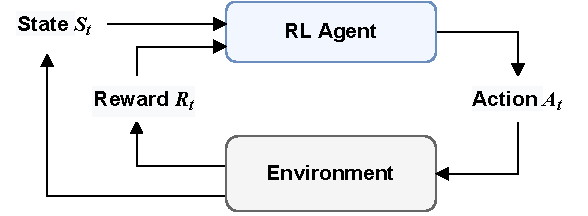
\includegraphics[width=0.5\textwidth]{RL-loop.pdf}
	\caption{Reinforcement Learning}
	\label{fig:RL-loop}
\end{figure}

Introduced in 1992, the REINFORCE algorithm \citep{REINFORCE-williams1992} is an early policy based RL algorithm, capable of handling both discrete and continuous observation and action spaces. In practice the REINFORCE algorithm is considered as a ``weak'' algorithm and superseded by several algorithms developed since. Most notably the deep-neural network version of Q-Learning, the Deep Q-Network (DQN) \citep{DQN-mnih2013}, followed by Actor-Critic \citep{A2C-mnih2016} and one of the most robust modern-day algorithms, the Proximal Policy Optimization (PPO) \citep{PPO-schulman2017}, Fig. \ref{fig:TimeLine}.
\begin{figure}[h]	
	\startchronology[startyear=1940, startdate=false, stopdate=false, arrow=false, color=codegray, height=.5ex]
	\chronoevent[textwidth=2.25cm]{1947}{Monte Carlo\endgraf \texttt{    }sampling}
	\chronoevent[markdepth=-20pt]{1959}{TD Learning}
	\chronoevent{1989}{Q-Learning}
	\chronoevent[markdepth=-20pt]{1992}{\textcolor{blue}{REINFORCE}}
	\chronoevent{2013}{DQN}
	\chronoevent[markdepth=-20pt]{2016}{A2C}
	\chronoevent[markdepth=50pt]{2017}{PPO}
	\stopchronology
	\vspace{-36pt}
	\caption{Time line of significant RL algorithms}
	\label{fig:TimeLine}
\end{figure}

\hlc{Our study takes a fresh look} at REINFORCE, an otherwise neglected algorithm since it is considered an early, na\"ive algorithm, comparing it against three advanced algorithms, namely, DQN, Advantage Actor-Critic (A2C), and PPO. Secondly, while most RL studies are evaluated on Open AI Gym environments, our experiments cover the predictive maintenance problem using a custom built environment. In practice the milling tool is replaced after a set threshold. We use this ``deterministic preventive maintenance'' policy as the baseline for comparing the various policies. Our systematic evaluation, based on levels of environment difficulty, different bench-mark datasets and varying noise levels allow a broader comparison of the algorithms. Finally, we conduct statistical tests to ensure a robust statistical-evidence based conclusion.

The main \textbf{contributions} of this research are:
\begin{enumerate}
	\item Contributes to the broader goal of AutoML for PdM, using RL.
	\item Research targeted toward the industrial practitioner not accustomed to complex hyper-parameter tuning of RL algorithms.
	\item Design and implement an RL environment for PdM of a milling machine.
	\item Rigorous evaluation of four standard, untuned , RL algorithms.
	\item Use of simple performance evaluation statistical measures and plots that industrial practitioners are normally used to.
\end{enumerate} 

The rest of the paper is structured as follows: In the next section we survey some related work and provide the necessary technical background describing the algorithms studied in this research. Section \ref{sec:Method} discusses implementation details of the REINFORCE algorithm and the predictive maintenance environment followed by the methodology adopted for training, testing and evaluation. Section \ref{sec:Results} and \ref{sec:Discussion} present and discuss, the results of experiments. Finally, we summarize and draw conclusions in Section \ref{sec:Conclusion}.

\section{Related work and background}\label{sec:SLR}
\subsection{Literature Review}
Significant work has been conducted in the application of RL for predictive maintenance in general \citep{Panzer2021, Erhan2021, siraskar2023}; however none of them covered\footnote{Query: \texttt{(milling OR "tool wear") AND "reinforcement learning" AND maintenance}. As of: 10-Jul-2023, across IEEE Xplore\texttrademark{}, Scopus\texttrademark{} and Web Of Science\texttrademark{}} PdM for milling machines. % $$$Note: 1 article returned (\cite{dai2021reinforcement}) is NOT predictive maintenance - but clamping position optimization. 
Similarly, automated machine learning (AutoML) for predictive maintenance was presented in only 9 research articles, with a coverage limited to supervised machine learning and therefore excluded RL. %\cite{AutoML-Larocque} use signal processing to standardize data followed by AutoML to select top performing models. \cite{AutoML-Hadi} use AutoML to accurately identify various types of faults in ball bearings, while \cite{AutoML-Maurer} has studied use of AutoML on log-data generated by production lines for performing preventive maintenance.  

%While RL is not, traditional machine learning methods \textit{have} been applied; for example \cite{Qin2023} and \cite{Qiang2023} apply tool wear law and physics based models before applying ML. \cite{Twardowski2023} and \cite{Denkena2023} use data gathered by sensors. While \cite{Twardowski2023} use two different classification trees, \cite{Denkena2023} use data recorded on other similar machines for building ML models. \cite{oshida2023development} proposes real-time tool wear detection using a stacked LSTM\footnote{long short-term memory networks} encoder-decoder model for anomaly detection as a mechanism to address predictive maintenance.  

Experimental comparison and analysis of various RL algorithms, has been limited to using standard benchmark OpenAI Gym environments. \cite{sandeep2022experimental} documents experimental evaluation of four policy-gradient and actor-critic algorithms PPO, SAC, DDPG and A2C using the Pendulum, Mountain Car, Bipedal Walker, Lunar Landing and Atari 2600 game environments. \cite{Krishna2020} evaluate DQN, DoubleDQN, A2C, REINFORCE and PPO using Cartpole, Space Invaders and the Lunar Lander. \cite{dulac2021, dulac2020empirical} are significant contributions toward analyzing empirical studies directed toward \textit{real-world} challenges. They apply real-world design concepts on the Cartpole and other complex environments such as humanoids and walkers from the Real-World Reinforcement Learning (RWRL) Suite\footnote{Link to RWRL >> \href{https://github.com/google-research/realworldrl_suite}{link}}. These environments are then evaluated for multiple algorithms such as, REINFORCE, Trust Region Policy Optimization (TRPO) and Deep Deterministic Policy Gradient (DDPG). 

\cite{dulac2021, henderson2018deep} tackle RL for continuous control. \cite{henderson2018deep} evaluate DDPG, ACKTR, TRPO and PPO on complex MuJoCo\footnote{\href{https://mujoco.org/}{MuJoCo} provides environments for studying Multi-Joint dynamics with Contact} environments such as the HalfCheetah, Hopper, Walker and Swimmer. Similar to our research, they used the OpenAI baseline implementations of RL algorithms for the experiments and evaluation. \cite{ford2022cognitive} is one experimental evaluation we found based on a \textit{real-world} application where DQN, A2C and PPO are applied for choosing the operational radio frequency (RF) mode for a multi-function RF system and go on to suggest that PPO is the best.

Our survey shows that most existing work use standard OpenAI Gym environments, which although necessary for bench-marking performance, do not provide coverage of industrial PdM. In Section \ref{sec:Implementation} we attempt to bridge this gap by implementing a custom built environment.

\subsection{Technical Background}
\subsubsection*{Key concepts of RL}
A task is a goal we set for our agent to learn. In our case the agent must learn to optimally predict the replacement of the tool. Frequent tool replacement increases down-time while delaying it results in inferior work piece quality. In Fig. \ref{fig:RL-loop} the agent interacts with the environment by performing an action ($a \in \mathcal{A}$), which then alters the state of the environment to one of many states ($s \in \mathcal{S}$). The resulting state is determined by a state-transition probabilities ($\mathcal{P}$) since RL is founded on Markov Decision Process (MDP) theory. The new state provides a feedback via a reward ($r \in \mathcal{R}$). Higher positive rewards ``reinforce'' good behavior. Performing this over thousands of episodes with the objective of maximizing the total rewards $R$, enables the agent to develop a policy $\pi$ which is essentially a mapping of the optimal action to perform given a certain state.

A \textbf{value function} computes how good a state or an action is by predicting future rewards, also known as a ``return'' $G_t = R_{t+1} + \gamma R_{t+2} + \dots = \sum_{k=0}^{\infty} \gamma^k R_{t+k+1}$. $\gamma \in [0, 1]$ facilitates discounting i.e. applying less weight to future rewards. Value functions can be represented by \textbf{state-value} $V_{\pi}(s)$ of a state $s$, as the expected return: $V_{\pi}(s) = \mathbb{E}_{\pi}[G_t \vert S_t = s]$; or an \textbf{action-value} function of a state-action pair as $Q_{\pi}(s, a) = \mathbb{E}_{\pi}[G_t \vert S_t = s, A_t = a]$.

With a brief overview of RL, we now briefly touch upon the core ideas of the four algorithms we experimented with.

\subsubsection*{Deep Q-Network (DQN)}
Deep Q-Network \citep{DQN-mnih2013} significantly improved the earliest RL algorithm, Q-learning, by introducing neural networks to learn policies for high-dimension environments with two novel strategies to significantly stabilize learning -- an ``experience replay buffer'' and a target network that was frozen and only periodically updated. Equation (\ref{eq:DQN}) shows the DQN loss function where $D$ is the replay memory and is sampled using a uniform distribution $U(D)$, $Q(s, a; \theta)$ is the function parameterized with $\theta$, that helps compute the Q values and $\theta^{-}$represents parameters of the frozen target Q-network.

\begin{equation}
	\mathcal{L}(\theta) = \mathbb{E}_{(s, a, r, s') \sim U(D)} \Big[ \big( r + \gamma \max_{a'} Q(s', a'; \theta^{-}) - Q(s, a; \theta) \big)^2 \Big]
	\label{eq:DQN}
\end{equation}

\subsubsection*{Advantage Actor Critic (A2C)}

A2C is a variant of Asynchronous Advantage Actor Critic (A3C) \citep{A2C-mnih2016}, and uses multiple computation workers to avoid the use of a replay buffer. A2C is a policy-gradient actor-critic algorithm. The policy-gradient family of algorithms strive to model and optimize the policy directly. Actor-critic structures consist of two networks -- a critic that updates function parameters $w$ of the value function (i.e either $Q_w(a \vert s)$ or $V_w(s)$); and an actor that updates the policy parameters $\theta$for $\pi_\theta(a \vert s)$, following the direction computed by critic. Actors therefore learn the parameterized policy $\pi_{\theta}$ using the policy-gradient as shown in (\ref{eq:A2C}). 
\begin{equation}
	\nabla_ \theta J(\pi_\theta) = \mathbb{E}_t \; [ \; A^\pi_t \; \nabla_\theta \ln \pi_\theta(a_t \vert s_t) \;]
	\label{eq:A2C}
\end{equation}
Where the advantage function $A^\pi_t (s_t, a_t)$ measures how good or bad the action is w.r.t. policy's average, for a particular state, using (\ref{eq:A2CAF}).
\begin{equation}
	A^\pi_t (s_t, a_t) = Q^\pi (s_t, a_t) - V^\pi (s_t)
	\label{eq:A2CAF}
\end{equation}

\subsubsection*{Proximal Policy Optimization (PPO)} 
\cite{PPO-schulman2017} formulated PPO which is often considered as the most robust of the RL algorithms. PPO is a policy-gradient method based on TRPO (Trust region policy optimization) by \cite{TRPO-schulman2015}, where the main idea is the use of a trust region to improve training stability by avoiding updates to parameters that vastly change the policy at a particular time step. TRPO ensures this by using a divergence constraint on the magnitude of policy update. If $r(\theta)$ (\ref{eq:rPPO}) represents the ratio of probabilities between policies of previous and current iteration, then the objective function of TRPO is given by (\ref{eq:TRPO}), where $\hat{A}$ represents the estimated advantage function.
\begin{equation}\label{eq:rPPO}
	r(\theta) = \frac{\pi_\theta(a \vert s)}{\pi_{\theta_\text{old}}(a \vert s)}
\end{equation}
\begin{equation}\label{eq:TRPO}
	J^\text{TRPO} (\theta) = \mathbb{E} [ r(\theta) \hat{A}_{\theta_\text{old}}(s, a) ]
\end{equation}

PPO extends TRPO by additionally imposing a regional constraint. It prevents large updates by forcing the ratio $r(\theta)$to stay within a small interval $[1-\epsilon, 1+\epsilon]$, around $1.0$, by use of a hyper-parameter $\epsilon$.
\begin{equation}
	J^{CLIP} (\theta) = \mathbb{E}_t \; [ \; min (r_t(\theta) A^{\pi_{\theta_{old}}}_t, clip(r_t(\theta), 1-\epsilon, 1+\epsilon) A^{\pi_{\theta_{old}}}_t)]
	\label{eq:PPO}
\end{equation}

\subsubsection*{REINFORCE} 
The REINFORCE algorithm, invented by \cite{REINFORCE-williams1992}, is an early algorithm that directly learns a policy $\pi_\theta$ to produce action probabilities from states. Actions that cause favorable states, are positively reinforced thereby increasing their probability of occurrence. Conversely, those resulting in unfavorable states are penalized.

The objective function (\ref{eq:REINFORCE-obj}) that the agent attempts to maximize is defined as the expected return over many trajectories sampled from the policy.
\begin{equation}\label{eq:REINFORCE-obj}
	\max_{\theta} J(\pi_{\theta}) = \mathop{\mathbb{E}}_{\tau \sim \pi_\theta} [R(\tau)]
\end{equation}

REINFORCE uses policy gradient (\ref{eq:REINFORCE}) to update the action probabilities.
\begin{equation}
	\nabla_ \theta J(\pi_\theta) = \mathbb{E}_t \; [ \; R_t(\tau) \; \nabla_\theta \ln \pi_\theta(a_t \vert s_t) \;]
	\label{eq:REINFORCE}
\end{equation}

\section{Methodology}\label{sec:Method}
\subsection{Implementation details}\label{sec:Implementation}
RL requires an environment to function. In this section we describe the custom milling environment we built, which allows our agent to learn a policy for tool replacement. Fig. \ref{fig:environments} shows the stepped approach used to generate the fifteen environments, of varying complexity. We next describe each variant starting with the simulation-based, followed by real-data based; describing their sub-variants along the way.
\begin{figure}[h]
	\centering
	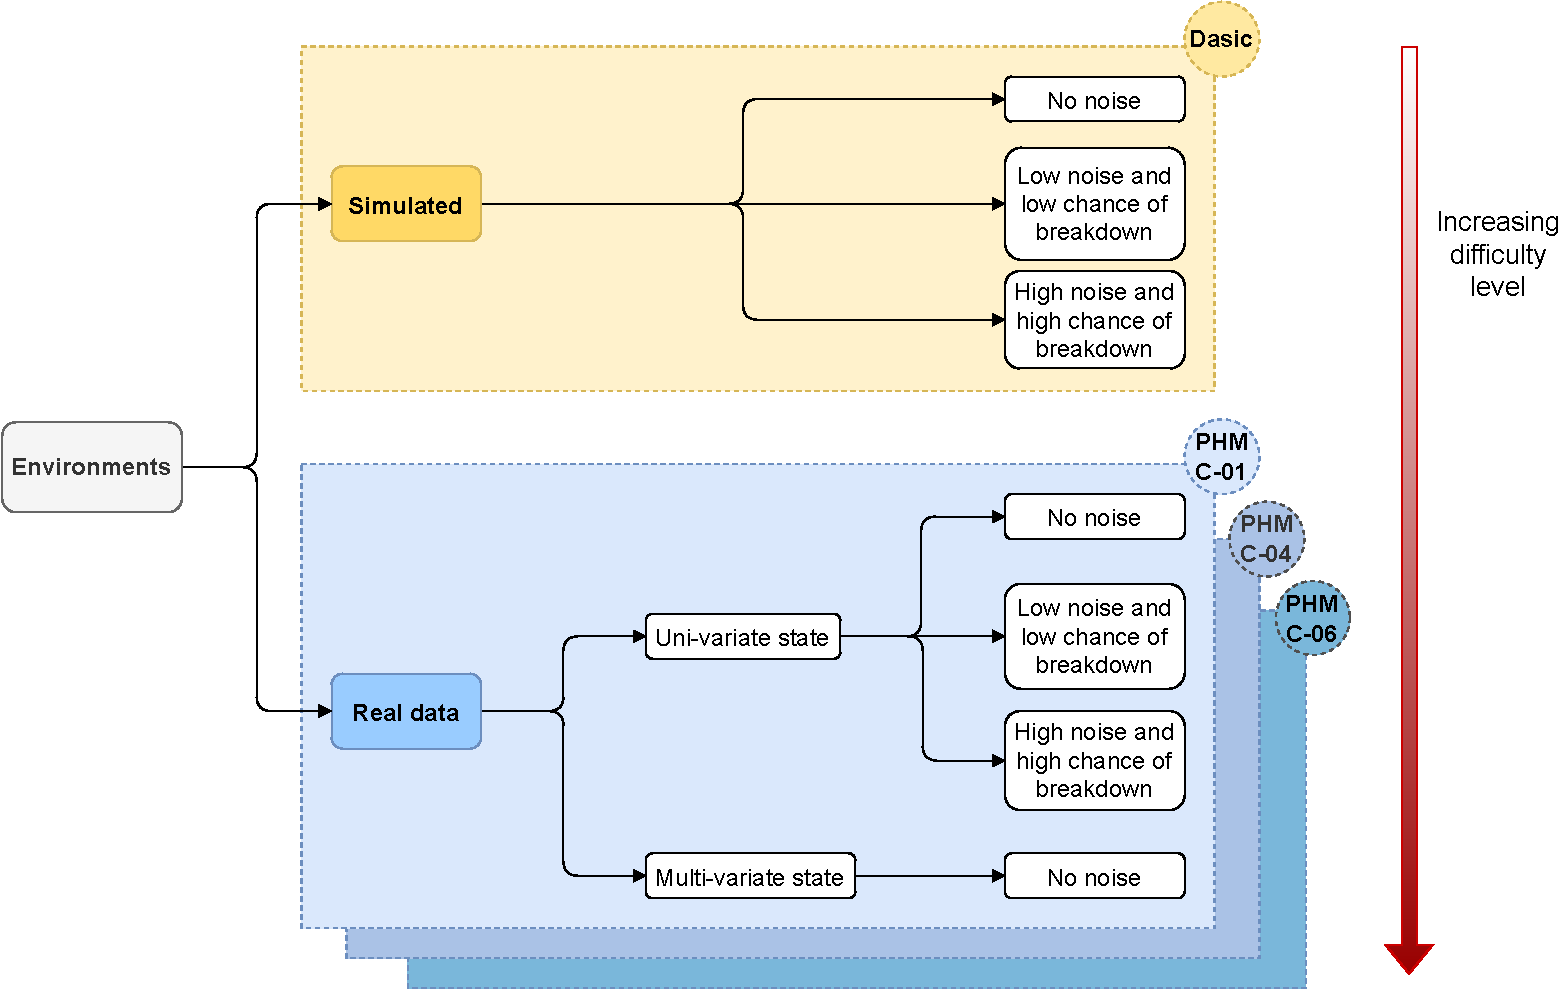
\includegraphics[width=0.8\textwidth]{Environments.pdf}  
	\caption{The fifteen different environments used for evaluation.}
	\label{fig:environments}
\end{figure} 

\begin{figure}[h]
	\begin{subfigure}[b]{0.5\textwidth}
		\centering
		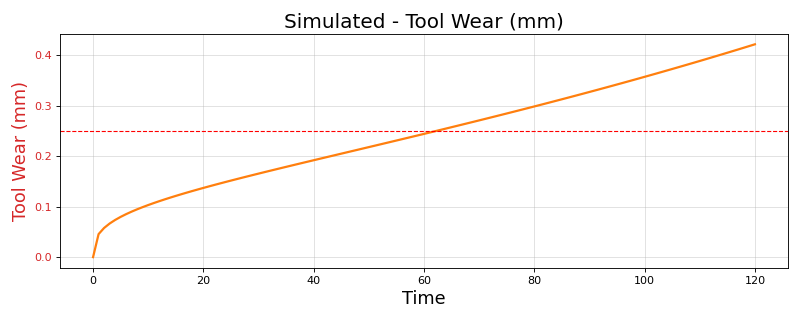
\includegraphics[width=\textwidth]{Simulated_wear_plot.png}  
		\caption{Simulated wear data}
		\label{fig:simulated}
	\end{subfigure}
	\hfill
	\begin{subfigure}[b]{0.5\textwidth}
		\centering
		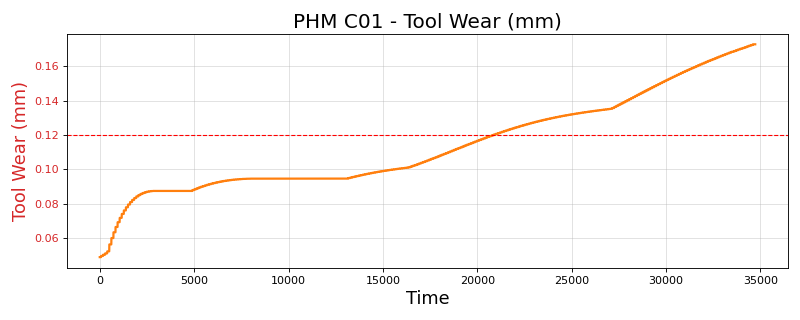
\includegraphics[width=\textwidth]{PHM_C01_wear_plot.png}  
		\caption{PHM C01 wear data}
		\label{fig:C01}
	\end{subfigure} \par\bigskip
	
	\begin{subfigure}[b]{0.5\textwidth}
		\centering
		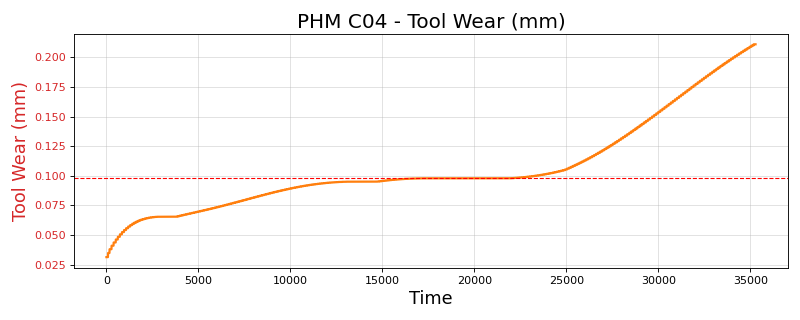
\includegraphics[width=\textwidth]{PHM_C04_wear_plot.png}  
		\caption{PHM C04 wear data}
		\label{fig:C04}
	\end{subfigure}
	\hfill
	\begin{subfigure}[b]{0.5\textwidth}
		\centering
		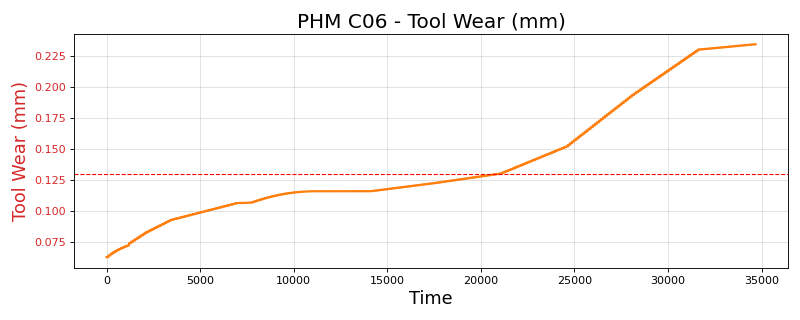
\includegraphics[width=\textwidth]{PHM_C06_wear_plot.png}  
		\caption{PHM C06 wear data}
		\label{fig:C06}
	\end{subfigure} 
	\label{fig:tool wear-plots}
	\caption{Tool wear data. Red dotted line indicates the wear threshold beyond which tool is replaced.}
\end{figure}

\subsubsection*{Simulating tool wear}
\cite{dasic2006} provides a parameterized power-exponential function for modeling tool wear \eqref{eq:Dasic}, where $VB$ represents the flank wear in mm.
\begin{equation}
	VB = a \cdot t^{b_1} \cdot e^{b_2 \cdot t} \Big|_{t=t_0}^{t=t_1}
	\label{eq:Dasic}
\end{equation}

We used the parameter values provided in the paper $a=0.08257$, $b1=0.3342$ and $b2=0.03147$ to simulate 120 data points. Fig. \ref{fig:simulated} shows the tool wear simulated using \eqref{eq:Dasic}, with the red dotted-line indicating the wear threshold beyond which tool is replaced. This provided the mechanism to simulate the basic variant of tool-wear based \textbf{univariate state}. We then added two further levels of increased complexity using noise and a chance of breakdown, giving us three distinct environments. 

\subsubsection*{Actual tool wear data}\label{sec:PHMdata}
The IEEE\textit{DataPort} hosts the ``2010 PHM Society'' tool-wear data obtained from a high-speed CNC milling machine, \citep{PHM-dataset}. C01, C04 and C06 datasets are suggested as benchmarks to be used for machine learning research and were the ones we used\footnote{In the article, we often refer to these datasets as ``PHM-'' data.}. The data is from seven sensors -- dynamometer measuring forces in X, Y and Z dimensions, measured in $N$; accelerometer measuring vibration in X, Y and Z dimensions, measured in $g$ and finally acoustic emission data as AE-RMS, in $V$. A separate file contains tool wear data in $mm$. Figures \ref{fig:C01}, \ref{fig:C04} and \ref{fig:C06} show the tool wear for the three datasets. We use real data to create two state designs, an univariate state consisting of only the tool wear and a \textbf{multivariate} state designed using all the additional seven sensor values. Just as we did for the simulated case, the complexity of the univariate state is increased using two levels of noise and break-down parameters. The multivariate state is complex in itself, Fig. \ref{fig:PHMMSdata}, and we use the natural (without noise) form.

\begin{figure}[h]
	\centering
	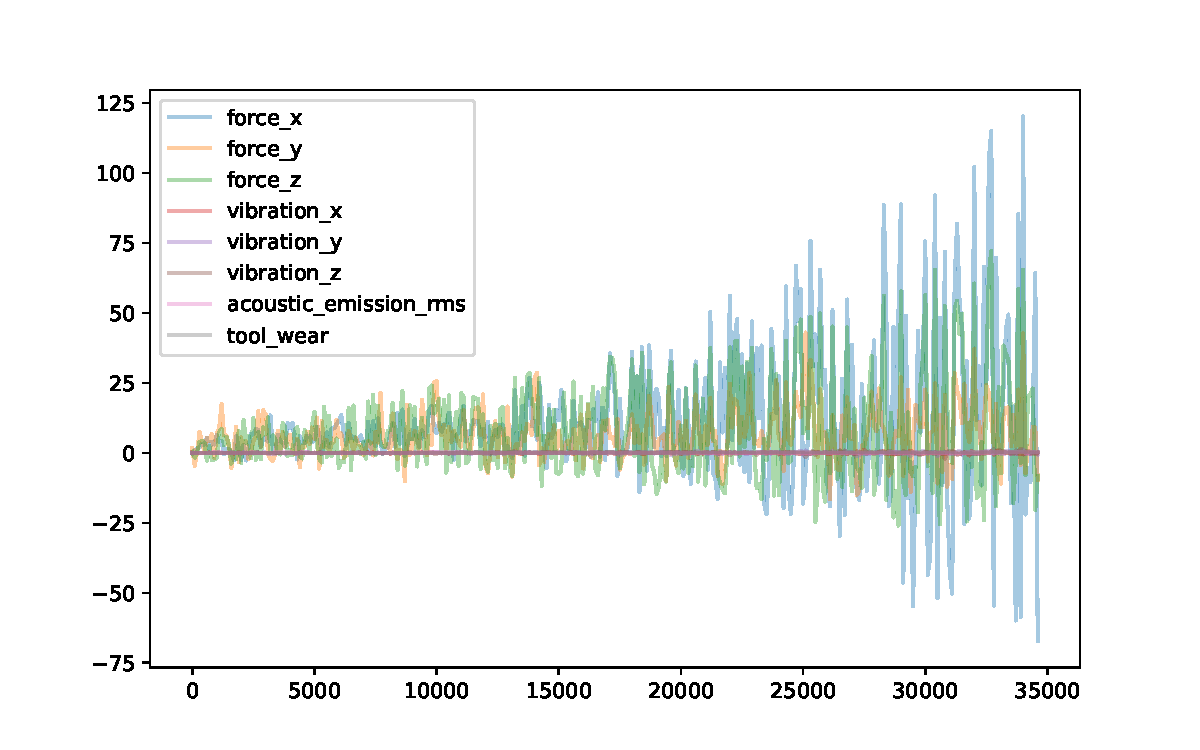
\includegraphics[width=0.7\textwidth]{PHMMSdata.pdf}  
	\caption{PHM C06: multivariate data}
	\label{fig:PHMMSdata}
\end{figure} 

In practice, state variables are often normalized to improve stability and convergence. Both the simulated and real data was normalized using min-max scaling such that the tool wear and other state features, $x \in [0,\;1] \subset \mathbb{R} $. We will see next how this allows adding white noise of similar magnitudes across different PHM datasets.

\subsubsection*{Adding noise and chance of break-down}
Fig. (\ref{fig:noise}) shows the effect of adding two levels of noise. ``Low noise'' is obtained by adding Gaussian noise with an order of magnitude of $-3$ i.e. $[0.0, 0.001]$ and ``high noise'' is of order $-2$ i.e. between $[0.0, 0.01]$. Since the tool wear is less than 0.24 mm, this adds significant perturbations as seen in Fig. (\ref{fig:LBD}) and (\ref{fig:HBD}). The noise affects the tool replacement decision (solid blue line) around the replacement threshold (dotted red line). The \textit{human} preventive maintenance policy replaces the tool if the wear exceeds the threshold and this decision boundary oscillates due to the noise. One can see that in the case of no noise (Fig. \ref{fig:NBD}), the decision boundary is clean.

\begin{figure}[h]
	\begin{subfigure}[b]{\textwidth}
		\centering
		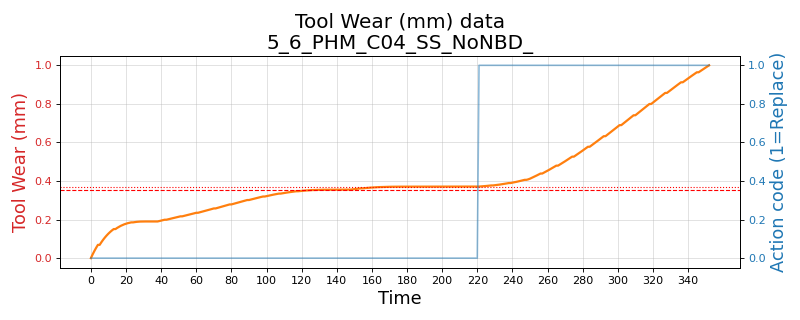
\includegraphics[width=0.65\textwidth]{PHM_C04_NoNBD_wear_plot.png}  
		\caption{No noise}
		\label{fig:NBD}
	\end{subfigure}
	\begin{subfigure}[b]{\textwidth}
		\centering
		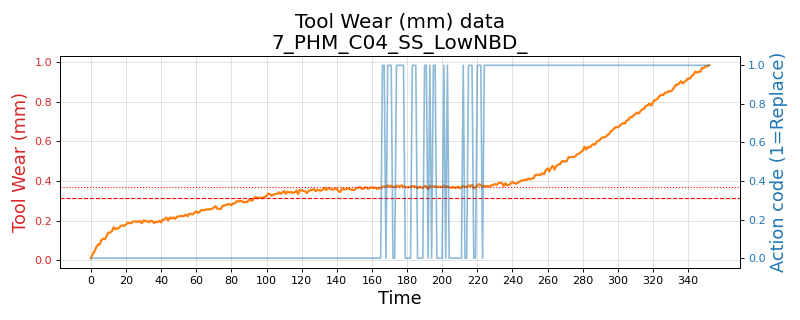
\includegraphics[width=0.65\textwidth]{PHM_C04_LowNBD_wear_plot.png}  
		\caption{Low noise}
		\label{fig:LBD}
	\end{subfigure}
	\begin{subfigure}[b]{\textwidth}
		\centering
		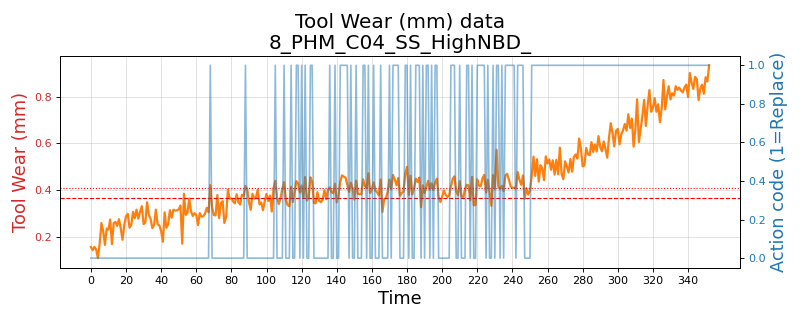
\includegraphics[width=0.65\textwidth]{PHM_C04_HighNBD_wear_plot.png}  
		\caption{High noise}
		\label{fig:HBD}
	\end{subfigure}
	\caption{PHM C04 tool wear data (normalized) and the effect of noise. Blue line is the replacement action decision.}
	\label{fig:noise}
\end{figure}

Break down occurs due to excessive tool use and can often occur randomly. In conjunction with Guassian noise this complexity is added for the univariate state based environments. For the low-noise variant we add a low 5\% chance of break down and for the high noise variant we add a higher chance of 10\%. The ``milling'' episode is terminated if a probability, sampled from a uniform distribution is less than this ``chance'' threshold.

Table \ref{tbl:ListEnvironments} summarizes the 15 environment variants and their three logical groups: (1) Simulated 1-3 (2) Real data -- simple univariate environment (4-12) and Real data -- complex multivariate (13-15).

\begin{table*}
	\sffamily
	\rowspace{1.3}
	\begin{tabular}{@{}r l rr@{}} \arrayrulecolor{black!40}\toprule 
		 & Environment variant & Noise factor & Breakdown chance \\ \midrule
		 & \multicolumn{3}{l}{\textbf{Simulated}}\\
		1 & Simulated - No noise  & None & None \\
		2 & Simulated - Low noise & 1e-3 & 0.05 \\
		3 & Simulated  - High noise & 1e-2 & 0.10 \\ \midrule
		\rule{0pt}{1.5\normalbaselineskip}
		 & \multicolumn{3}{l}{\textbf{Real data -- simple univariate}} \\
		4 & PHM C01 SS (simple, univariate) - No noise & None & None \\
		5 & PHM C01 SS (simple, univariate) - Low noise & 1e-3 & 0.05 \\
		6 & PHM C01 SS (simple, univariate) - High noise & 1e-2 & 0.10 \\ \hdashline
		
		7 & PHM C04 SS (simple, univariate) - No noise & None & None \\
		8 & PHM C04 SS (simple, univariate) - Low noise & 1e-3 & 0.05 \\
		9 & PHM C04 SS (simple, univariate) - High noise & 1e-2 & 0.10 \\ \hdashline
		
		10 & PHM C06 SS (simple, univariate) - No noise & None & None \\
		11 & PHM C06 SS (simple, univariate) - Low noise & 1e-3 & 0.05 \\
		12 & PHM C06 SS (simple, univariate - High noise & 1e-2 & 0.10 \\ \midrule
		
		\rule{0pt}{1.5\normalbaselineskip}
		& \multicolumn{3}{l}{\textbf{Real data -- complex multivariate}}\\
		13 & PHM C01 MS (complex, multivariate) - No noise & None & None \\
		14 & PHM C04 MS (complex, multivariate) - No noise & None & None \\
		15 & PHM C06 MS (complex, multivariate) - No noise & None & None \\ \bottomrule
	\end{tabular}
	\caption{List of the fifteen environments and their categorization}
	\label{tbl:ListEnvironments}
\end{table*}

\subsubsection*{Tool wear as a Markov Decision Processes (MDP)}
Formulating our problem to be solved by RL requires us to assume that the wear process satisfies the Markov property -- which implies that the transition of tool wear to another state is dependent only on the current state and not on any previous states. MDPs are defined by the tuple $<\mathcal{S, A, P, R, \gamma}>$. We will define the elements of state space $\mathcal{S}$, action space $\mathcal{A}$ and reward function $\mathcal{R}$, next.

\subsubsection*{State and environment elements}
There are two basic state definitions across the 15 environment variants, the ``simple univariate'' and the ``complex multivariate''. 

The elements of simple univariate state vector are $S_t = [w_t]$, where $w_t$ is the current tool wear. As part of the environment other elements that are sensed by the agent are $[W_\tau, N_f, P_{bd}]$, where $W_\tau$is the wear threshold, $N_f$ is the noise factor and is one of [0, 1e-3, 1e-2], $P_{bd}$ is the chance of tool breakdown and is one of [0, 0.05, 0.10]. The complex multivariate state $S_t = [f_x, f_y, f_z, v_x, v_y, v_z, ae_{rms}, w_t]$ where, as mentioned in Section \ref{sec:PHMdata}, $(f_x, f_y, f_z)$ represents the force along the 3 axes, similarly $v$ represents the vibration, $ae_{rms}$ the acoustic emission.

\subsubsection*{Actions}
The action space is binary, $\mathcal{A} \in [0, 1]$, where $0$($\texttt{CONTINUE}$) represents continuation of milling operation and $1$($\texttt{REPLACE\_TOOL}$) represents the action of replacing the tool.

\subsubsection*{Environment feedback}
\hlc{``Feedback'' generated by the action an agent takes, is the central mechanism by which agents learn}. This is implemented via the \texttt{step()} function in the environment code and is outlined in Algorithm \ref{alg:SSStep}. At every time step an action $A_t$ is taken and the resulting state is evaluated for terminating conditions or assigning a reward and continuing.

\subsubsection*{Reward function}
\begin{equation}
	R_t \;\;=\;\;
	\begin{cases}
		\;\;  +R_1 \times t, & \quad if \;\; w_t < W_\tau\\
		\;\;  -R_2 \times t, & \quad if \;\; w_t\ge W_\tau\\
		\;\; \mathrel{+}= -R_3, & \quad if \;\; \text{ACTION = REPLACE\_TOOL}\\
	\end{cases}
	\label{eq:RewardFunction}
\end{equation}
In the reward function \eqref{eq:RewardFunction} there are three distinct phases where a reward (or penalty) is offered as feedback. $R_1$, $R_2$ and $R_3$ are constants that determine the magnitude of reward. When the current state of wear $w_t$ is less than the threshold $W_\tau$ we have a desirable condition, and we award the agent a positive reward. The formulation \eqref{eq:RewardFunction} allows a higher reward to be collected the closer it is to threshold so as to maximize tool usage, but not allowing it to cross it. If it does, the agent is penalized (negative reward) by a magnitude of $R_2$, and once again the farther away it is from the threshold i.e. a highly deteriorated tool the larger the penalty. To avoid this ``bad" state, the agent must learn to replace the tool; represented by the third condition. Tool replacement implies a direct cost (that of the tool) and a much higher and significant downtime ``cost''. To ensure the agent does not learn to replace unnecessarily, we ``penalize'' it. It is important to note that the last condition in \eqref{eq:RewardFunction} is an ``incremental addition'', the first two conditions are mutually exclusive and evaluated first, followed by the last condition which is incrementally added on whatever reward is collected in the previous condition. The agent then tries to balance these three conditions, such that it maximizes its total return, over time.

Of the final two elements of the MDP quintuple $\mathcal{P}$ represents the probability transition matrix and is usually not known and we will therefore use \textit{model-free} RL techniques to learn that from ``experiences''; $\gamma$ enables the agent to learn long-term impact of its actions i.e. what is the long term impact of replacing the tool now or that of delaying the replacement, $\gamma$ is set to 0.99 to facilitate this farsightedness.

\begin{algorithm}[h]
	\onehalfspacing
	\caption{Agent class \texttt{step()} method -- Reward handling mechanism}\label{alg:SSStep}
	\begin{algorithmic}[1]
		\Procedure {Step class method: Reward handling}{}\newline
		\textbf{Class attributes:} Wear-threshold $W_\tau$, reward accumulated so far $Reward$, reward function parameters $R1$, $R2$ and $R3$, random chance of breakdown $P_{bd}$, tool replacements made so far $tool_replacements$, maximum allowable operations $T$\newline
		\textbf{Input:} Current length of episode $t$, current tool-wear $w_t$, current policy action $A_t$,  current index of training data $data\_index$ \newline
		%\textbf{Output:} Predicted tool-wear values $\hat{y}$, computed attention weights $A$\newline
		
		\State \textbf{Initialize} $p$ from uniform probability distribution
		%\LineComment{Termination conditions: Terminate episode, reset reward values and reset\par 
		%				\hskip8pt the training data-frame index to the beginning.}
		%\If {length of episode $\geq$ maximum allowable operations}:
		
		\If {$t \geq T$}:
			\LineComment{Termination based on length of episode.}
			\State $Terminate \gets True$
			\State $Reward \gets 0.0$
			\State $data\_index \gets 0$	\Comment{Reset the training data-frame index to the beginning.}\newline
			
		%\ElsIf {tool-wear is $>$ wear threshold $W_\tau$ AND random-chance of breakdown $P_{bd} >$wear threshold $W_\tau$}
				
		\ElsIf {$w_t > W_\tau$ \textbf{and} $p < P_{bd}$}:
				\LineComment{Termination based on chance of breakdown.}
		
				\State $Terminate \gets True$
				\State $Reward \gets 0.0$
				\State $data\_index \gets 0$		
		\Else
			\State $Terminate \gets False$
			\If {$ w_t < W_\tau $}:
					\LineComment{Healthy tool}
					\State $Reward \gets Reward + t \cdot R1$
			\Else
				\LineComment{Tool deteriorating}
				\State $Reward \gets Reward - t \cdot R2$	
			\EndIf
			\If {$A_t$ is $REPLACE\_TOOL$}:
				\LineComment{Tool is replaced}
				\State $Reward \gets Reward - R3$
				\State $data\_index \gets 0$ \Comment{Tool replaced, therefore roll back tool life}
				\State Increment $tool\_replacements$
			\EndIf			
		\EndIf
		\EndProcedure
	\end{algorithmic}
\end{algorithm}

\subsubsection*{Network architecture and basic hyper-parameters}
Stable-Baselines3 (SB3) \cite{SB3-paper} provides robust open source implementations of many RL algorithms. As of 10-Jul-2023, 13 algorithms have been implemented \citep{SB3-algorithms} however REINFORCE has \textit{not} been implemented. For this research we use the \textit{default} SB3 implementations of DQN, A2C and PPO and compare its performance to a custom implementation of the REINFORCE algorithm using a very simple network architecture. Table \ref{tbl:network-architecture} shows a comparison of the architecture and the basic common hyper-parameters.
\begin{small}
\begin{table*}\centering
	\sffamily
	\rowspace{1.5}
	\begin{tabular}[htbp]{L{2cm} R{2.5cm} R{2.5cm} R{2.5cm} R{3cm}}
		\arrayrulecolor{black!40}\toprule
		&\textbf{A2C}&\textbf{DQN}&\textbf{PPO}&\textbf{REINFORCE}\\ \midrule
		
		Network\par architecture&input dim x\par [64|Tanh x 64|Tanh]\par x output dim&input dim x\par [64|Tanh x 64|Tanh]\par x output dim&input dim x\par [64|Tanh x 64|Tanh]\par x output dim&input dim x\par [64|ReLU]\par x output dim\\
		Layers&2&2&2&1\\
		Units&64  x 64&64  x 64&64  x 64&64\\
		Activation&Tanh, Tanh&Tanh, Tanh&Tanh, Tanh&ReLU\\
		Optimizer&RMSprop&Adam&Adam&Adam\\ \midrule
		Learning rate&0.0007&0.0001&0.0003&0.01\\
		Gamma&0.99&0.99&0.99&0.99\\			
		\bottomrule
	\end{tabular}
	\caption{Comparing the network architecture and basic hyper-parameters across algorithms}
	\label{tbl:network-architecture}
\end{table*}
\end{small}
The REINFORCE uses a \textit{single} internal layer of 64 units. The default architecture for all three SB3 algorithms (A2C/DQN/PPO) consists of \textit{two} fully connected layers with 64 units per layer \citep{SB3-DefaultNetwork}. While REINFORCE used ReLU (rectified linear unit) as the activation function, the other three algorithms used hyperbolic tangent (Tanh). Finally, REINFORCE's learning-rate is also much larger.

\subsection{Training}
The training strategy must ensure a uniform comparison of the algorithms. We maintained the exact \textit{same} environment variant, wear dataset, noise parameter, probability of breakdown parameter, and the three reward function parameters; across all four algorithms during a single training round. %Our code is fairly automated and we used a configuration file to configure the training experiments and record the test results. Fig. \ref{fig:exptconfig} shows the main columns of the configuration file we used.
As the wear data is time-series data, the training and test sets are created by systematic sampling. Simulated data and real tool wear data (PHM) was randomly sampled at a certain frequency and down sampled into training and test sets.
%\begin{figure}[ht]
%	\centering	
%	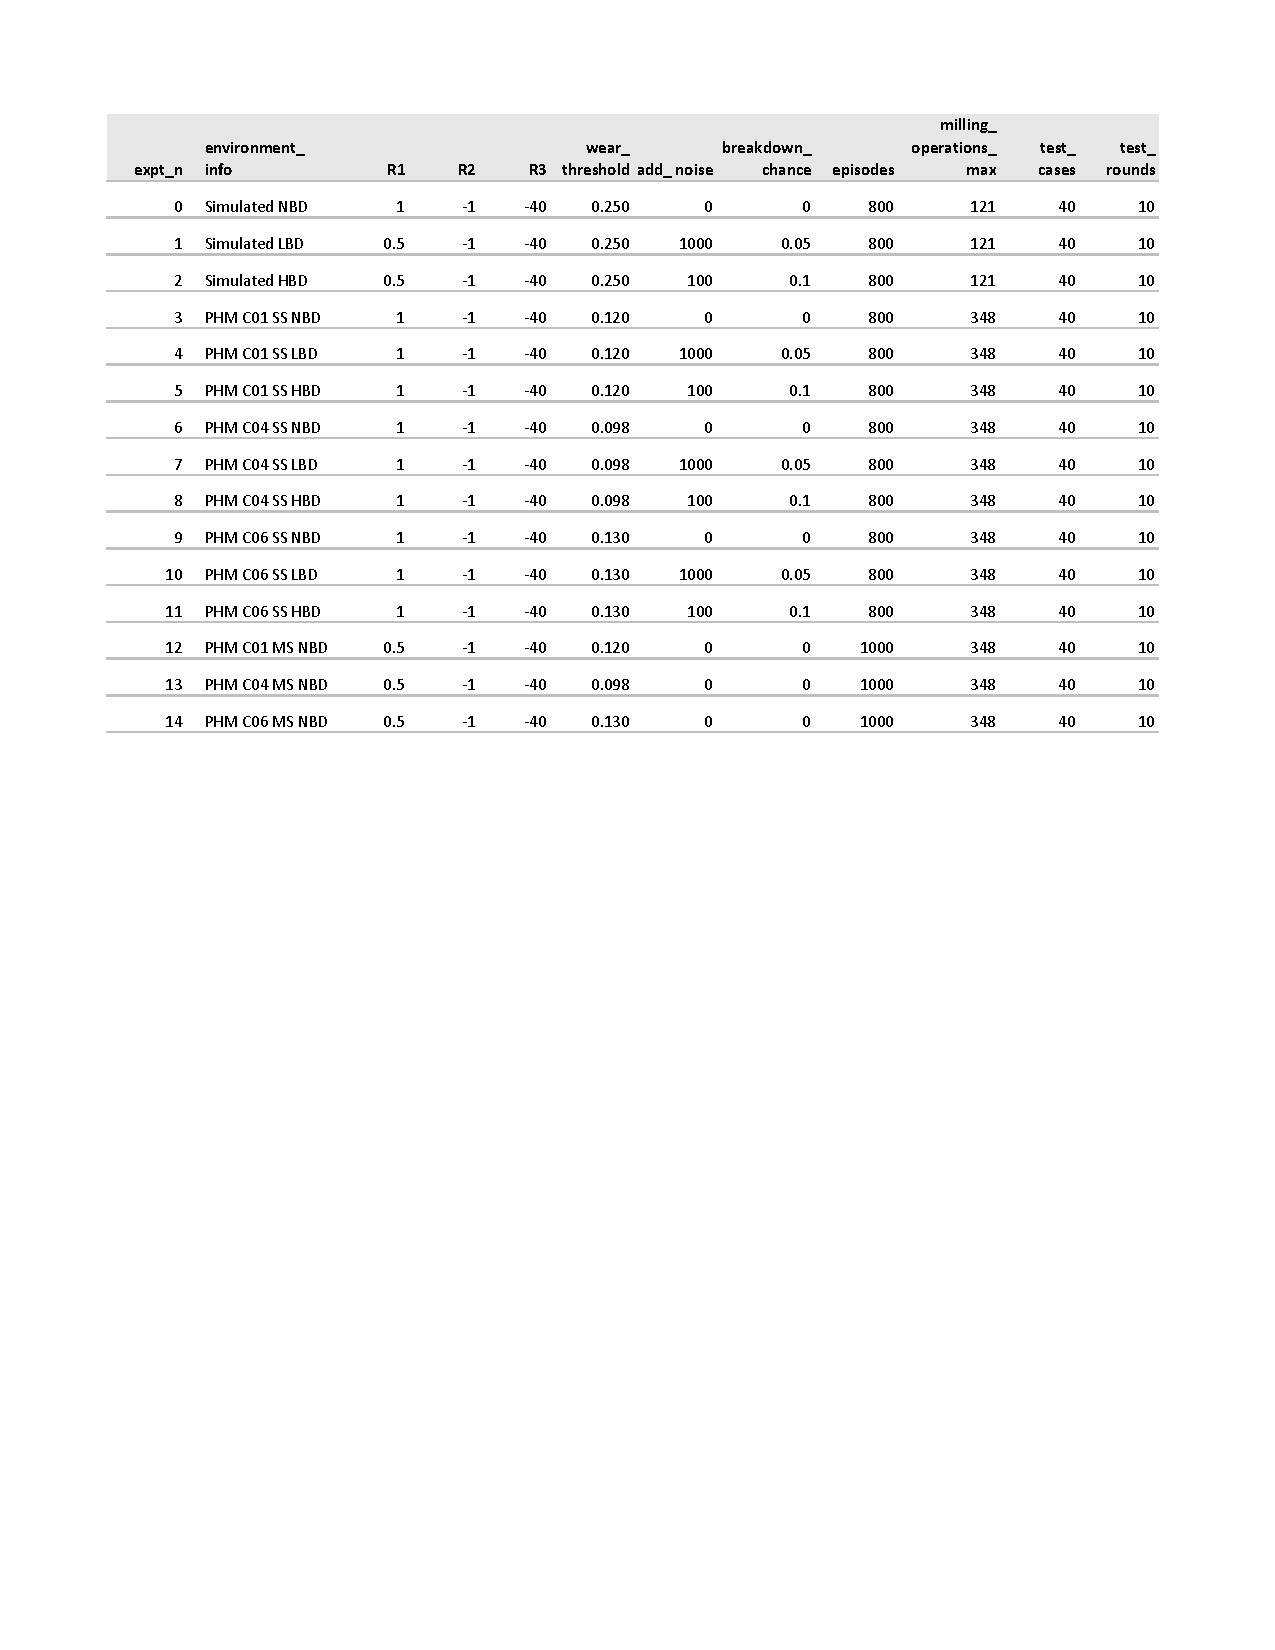
\includegraphics[width=\textwidth, trim={1.5cm 15cm 1cm 2cm}, clip]{images/TrainingPlots/Experiments_Sheet_select.pdf}  
%	\caption{Configuring the experiments}
%	\label{fig:exptconfig}
%\end{figure}

The REINFORCE was trained for 800 episodes for the simulated and PHM univariate variants, for all three noise and breakdown levels (none, low and high) -- Table \ref{tbl:ListEnvironments} items 1-12. For the PHM multivariate variant, Table \ref{tbl:ListEnvironments} items 13-15, REINFORCE was trained for 1000 episodes. SB3 algorithms were trained for 10,000 episodes for all variants. We ran ten rounds of training, tested each generated model and averaged results over the 10 rounds. Testing is explained in the next section while results are presented in Section \ref{sec:Results}.

\begin{figure}[h]
	\begin{subfigure}[b]{0.5\textwidth}
		\centering
		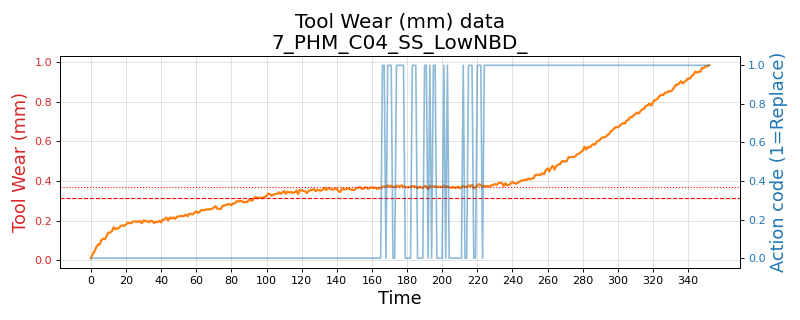
\includegraphics[width=\textwidth]{images/TrainingPlots/7_PHM_C04_SS_LowNBD__wear_plot.png}  
		\caption{PHM C04 wear data}
		\label{fig:C04wear}
	\end{subfigure}
	\hfill
	\begin{subfigure}[b]{0.5\textwidth}
		\centering
		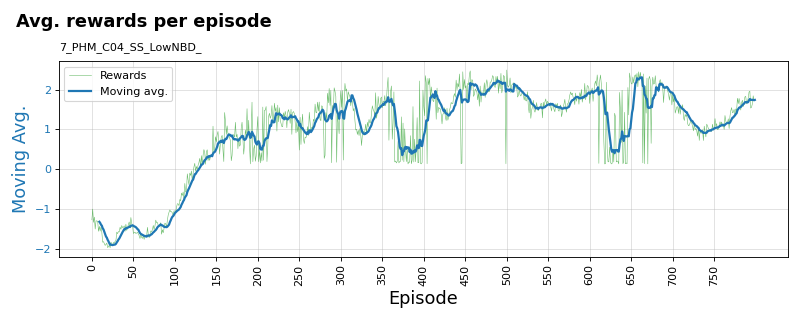
\includegraphics[width=\textwidth]{images/TrainingPlots/7_PHM_C04_SS_LowNBD__Avg_episode_rewards.png}  
		\caption{Average rewards per episode}
		\label{fig:C04rewards}
	\end{subfigure} \par\bigskip
	
	\begin{subfigure}[b]{0.5\textwidth}
		\centering
		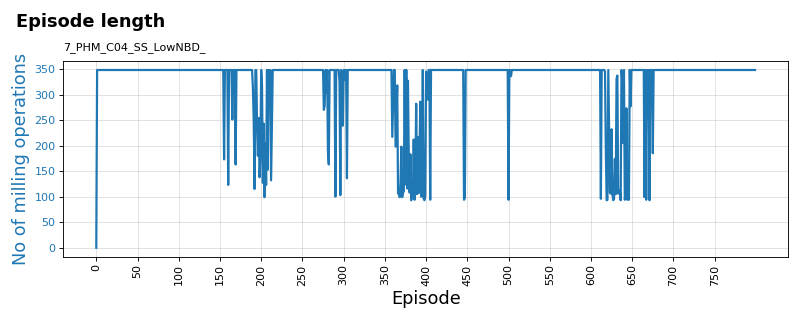
\includegraphics[width=\textwidth]{images/TrainingPlots/7_PHM_C04_SS_LowNBD__Episode_Length.png}  
		\caption{Episode length completed per episode}
		\label{fig:C04eplen}
	\end{subfigure}
	\hfill
	\begin{subfigure}[b]{0.5\textwidth}
		\centering
		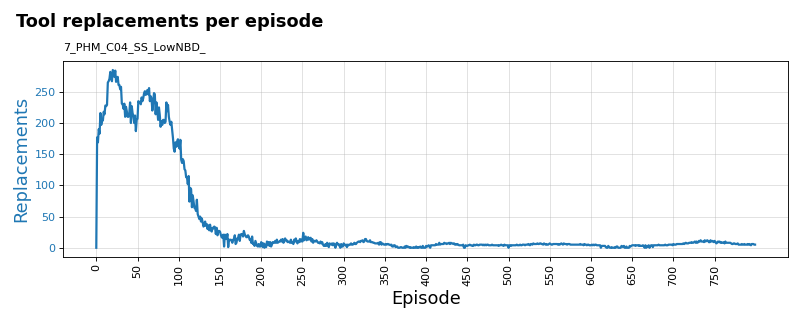
\includegraphics[width=\textwidth]{images/TrainingPlots/7_PHM_C04_SS_LowNBD__Tool_Replacements.png}  
		\caption{Tool replacements per episode}
		\label{fig:C04toolrep}
	\end{subfigure} 
	\caption{Training plots of REINFORCE. Dataset: PHM-C04. Variant: Univariate state, low-noise and low chance of breakdown.}
	\label{fig:C04trplots}
\end{figure}
Fig. \ref{fig:C04trplots} shows the training plots for the algorithm of our interest -- REINFORCE. It displays how the wear plot looked for C04 with low noise and low chance of breakdown settings. The average rewards increase over the course of 800 episodes (Fig. \ref{fig:C04rewards}). The episode length (Fig. \ref{fig:C04eplen}) demonstrates the complexity introduced by random breakdown (which abruptly terminates the episode). It is the tool replacement policy that is of interest to the industrial practitioner -- Fig. \ref{fig:C04toolrep} shows that it decreases to optimal levels as the agent learns over time. Similarly, Fig. \ref{fig:C06trplots} demonstrates the training for the PHM C06 dataset affected by high noise and higher breakdown probability. Finally, for the more complex multivariate state variant, the training plots are as seen in Fig. \ref{fig:C01trplots}; as we do not introduce noise or breakdown here, the episodes are always completed (Fig. \ref{fig:C01eplen}).

\begin{figure}[h]
	\begin{subfigure}[b]{0.5\textwidth}
		\centering
		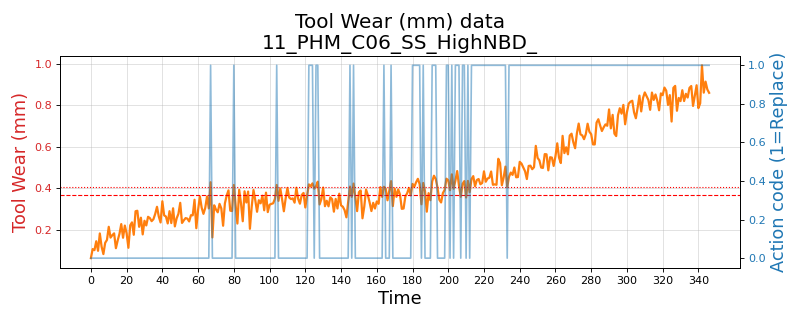
\includegraphics[width=\textwidth]{images/TrainingPlots/11_PHM_C06_SS_HighNBD__wear_plot.png}  
		\caption{PHM C06 wear data}
		\label{fig:C06wear}
	\end{subfigure}
	\hfill
	\begin{subfigure}[b]{0.5\textwidth}
		\centering
		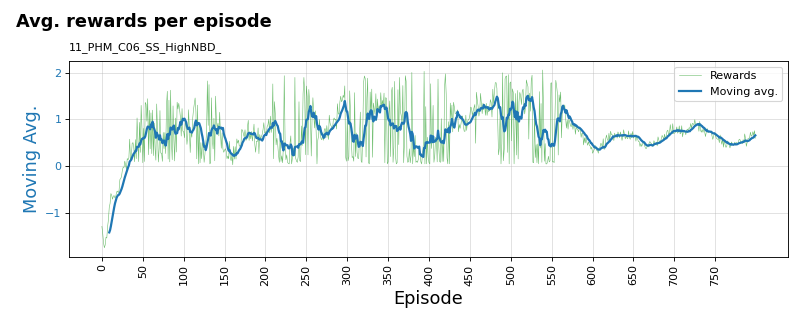
\includegraphics[width=\textwidth]{images/TrainingPlots/11_PHM_C06_SS_HighNBD__Avg_episode_rewards.png}  
		\caption{Average rewards per episode}
		\label{fig:C06rewards}
	\end{subfigure} \par\bigskip
	
	\begin{subfigure}[b]{0.5\textwidth}
		\centering
		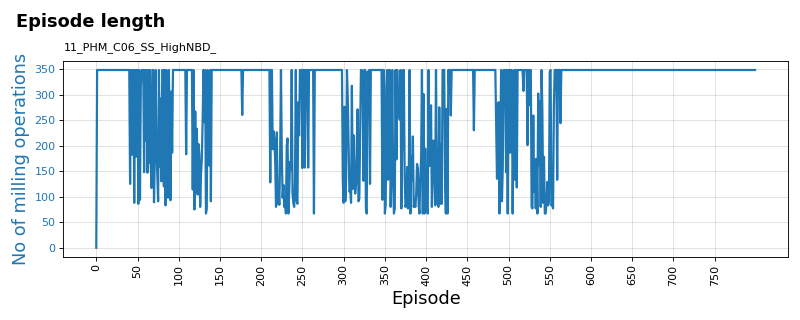
\includegraphics[width=\textwidth]{images/TrainingPlots/11_PHM_C06_SS_HighNBD__Episode_Length.png}  
		\caption{Episode length completed per episode}
		\label{fig:C06eplen}
	\end{subfigure}
	\hfill
	\begin{subfigure}[b]{0.5\textwidth}
		\centering
		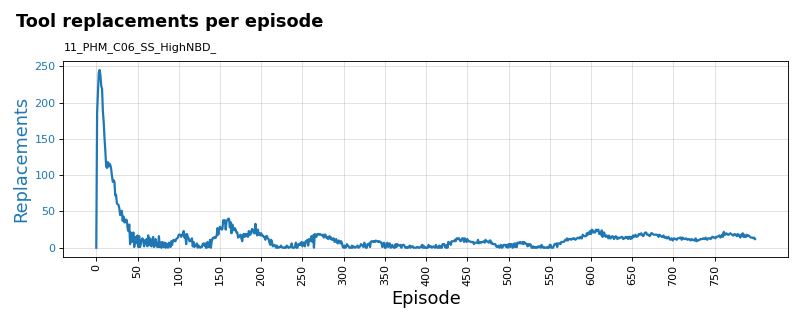
\includegraphics[width=\textwidth]{images/TrainingPlots/11_PHM_C06_SS_HighNBD__Tool_Replacements.png}  
		\caption{Tool replacements per episode}
		\label{fig:C06toolrep}
	\end{subfigure} 
	\caption{Training plots of REINFORCE. Dataset: PHM-C06. Variant: Univariate state, high-noise and high chance of breakdown.}
	\label{fig:C06trplots}
\end{figure}

\begin{figure}[ht]
	\begin{subfigure}[b]{0.5\textwidth}
		\centering
		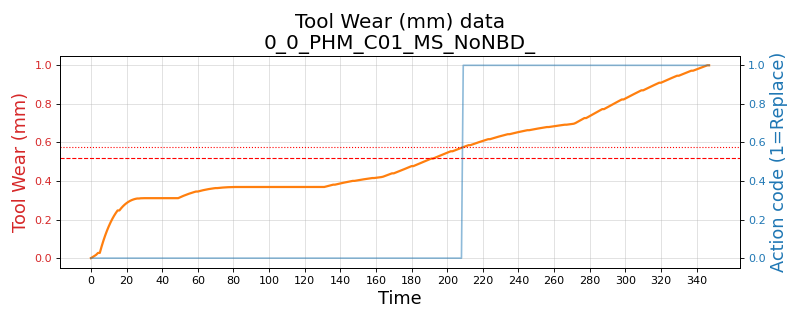
\includegraphics[width=\textwidth]{images/TrainingPlots/0_0_PHM_C01_MS_NoNBD__wear_plot.png}  
		\caption{PHM C01 wear data}
		\label{fig:C01wear}
	\end{subfigure}
	\hfill
	\begin{subfigure}[b]{0.5\textwidth}
		\centering
		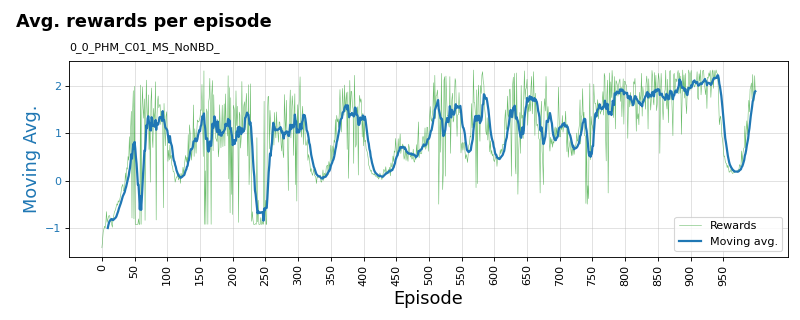
\includegraphics[width=\textwidth]{images/TrainingPlots/0_0_PHM_C01_MS_NoNBD__Avg_episode_rewards.png}  
		\caption{Average rewards per episode}
		\label{fig:C01rewards}
	\end{subfigure} \par\bigskip
	
	\begin{subfigure}[b]{0.5\textwidth}
		\centering
		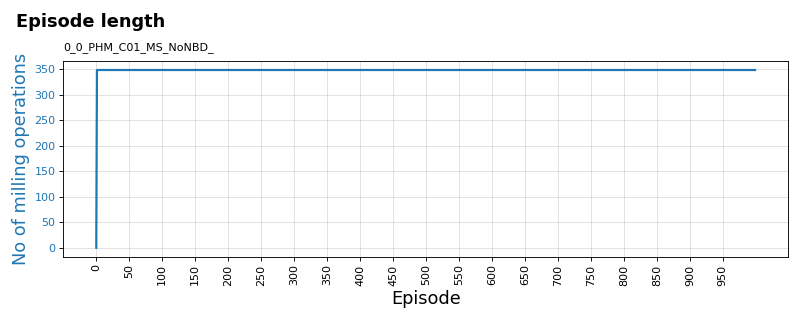
\includegraphics[width=\textwidth]{images/TrainingPlots/0_0_PHM_C01_MS_NoNBD__Episode_Length.png}  
		\caption{Episode length completed per episode}
		\label{fig:C01eplen}
	\end{subfigure}
	\hfill
	\begin{subfigure}[b]{0.5\textwidth}
		\centering
		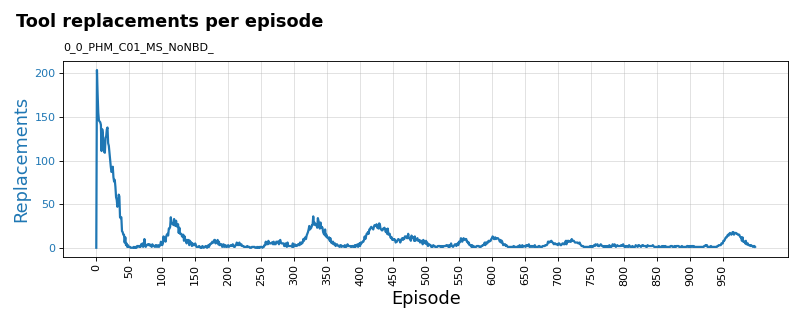
\includegraphics[width=\textwidth]{images/TrainingPlots/0_0_PHM_C01_MS_NoNBD__Tool_Replacements.png}  
		\caption{Tool replacements per episode}
		\label{fig:C01toolrep}
	\end{subfigure} 
	\caption{Training plots of REINFORCE. Dataset: PHM-C01. Variant: Multivariate state, No noise or breakdown.}
	\label{fig:C01trplots}
\end{figure}

\subsection{Testing and performance evaluation}
Testing was performed with data separate from the training data. 10 rounds of testing are performed, with a \textit{new} set of 40 test cases randomly sampled and frozen across all four algorithms, during each round.

\subsubsection*{Evaluation metrics}
The human decision is based on ``preventive maintenance'' -- replace the tool against a predefined wear threshold. In our data a tool replacement is represented as 1 and a normal operation as 0. We applied classification metrics to evaluate the RL agent decisions of tool replacement. %These are simple to understand for the general industrial practitioners against other RL evaluation methods such as average reward or the number of episodes to reach maximum reward. 
It is worth noting that while we have selected an arbitrary wear threshold as this serves our purpose for algorithm comparison; in reality the threshold is based on several factors like materials of tool and work-piece, the duration of continuous operation, ambient conditions, ``cost'' of production downtime etc. Threshold could therefore vary significantly from one case to another. 
\begin{figure}[h]
	\begin{center}
		\sffamily
		\rowspace{1.6}
		\begin{tabular}{l|l|c|c|}
			\multicolumn{2}{c}{}&\multicolumn{2}{c}{\textbf{Human decision}}\\
			\cline{3-4}
			\multicolumn{2}{c|}{}&Replace tool&Continue milling\\
			\cline{2-4}
			\multirow{2}{*}{\textbf{Agent decision}}& Replace tool & $TP$& $FP$\\
			\cline{2-4}
			& Continue milling& $FN$& $TN$\\
			\cline{2-4}
		\end{tabular}
	\end{center}
	\caption{Confusion matrix: Human versus Agent decisions}
	\label{fig:CM}	
\end{figure}

Classification metrics are based on the confusion matrix shown in Fig. \ref{fig:CM}. $TP$ represents true positive cases, where both the agent and human agree on replacing the tool. False positive $FP$ cases denote the agent falsely suggesting replacements, while false negatives $FN$ are cases where continuation of milling is suggested, when in fact a tool replacement would have helped. Precision (Pr), Recall (Rc) and F1-score metrics can then be computed as shown in \eqref{eq:metrics}.

\begin{equation}
	\text{Pr} = \frac{TP}{TP+FP}, \quad
	\text{Rc} = \frac{TP}{TP+FN}, \quad
	\text{F1-score} = 2 \times \frac{Pr \times Rc)}{(Pr + Rc)}
	\label{eq:metrics}
\end{equation}

\textbf{Tool replacement precision}: Timely replacements, $TP$, ensure work piece quality. While we desire high $TP$s, we do not want \textit{unnecessary} replacements which would otherwise and reduce costly production downtime, we therefore want lower $FP$s. The precision metric is therefore an ideal performance metric. 

While we prefer a high precision, we do want a reasonably high recall i.e. do not want to miss replacement opportunities (low $FN$s). The F1-score (true harmonic mean of precision and recall) gives us a \textit{balanced} measure. Equation (\ref{eq:Fbeta}) provides a \textit{weighted} mechanism to provide a higher F-score for higher precision, by setting $\beta < 1.0$. For our evaluation we set $\beta$ to $0.5$.

\begin{equation}
	F_{\beta} = (1+\beta^2) \cdot \frac{Pr \times Rc)}{(\beta^2 \cdot Pr + Rc)}
	\label{eq:Fbeta}
\end{equation}

%\begin{verbatim}
%	env = MillingTool_SS_NT(df_train, WEAR_THRESHOLD_NORMALIZED, MILLING_OPERATIONS_MAX, ADD_NOISE, BREAKDOWN_CHANCE, R1, R2, R3)
%	
%	env_test = MillingTool_SS_NT(df_test, WEAR_THRESHOLD_ORG_NORMALIZED, MILLING_OPERATIONS_MAX, ADD_NOISE, BREAKDOWN_CHANCE, R1, R2, R3)
%\end{verbatim}

\section{Results}\label{sec:Results}
\hlc{We present the summarized results in this section accompanied by commentary referring to detailed results made available in Appendix {\ref{apx}}. Since there are several tables and figures, for reference, we created a cross-linked Table {\ref{tbl:ref-results}}. Tables in this section and Appendix {\ref{apx}} use {\textcolor{dblue}{blue}} text to highlight prominent values. Plots accompany tables to assist in visualizing the comparative performance.}
\begin{table*}[h]\centering
	\sffamily
	\rowspace{1.3}
	\begin{tabular}{R{0.25cm} L{11.5cm} L{3cm}}
		\arrayrulecolor{black!40}\toprule 
		  & Results for & Numeric / Graphical\\ \midrule
		  \rowcolor{ltgray} & \textbf{Summary Results}  & \\ 
		1 & Overall summary -- All 15 environments, averaged over 10 rounds & Table \ref{tbl:OverallSummary}, Fig. \ref{fig:OverallSummary}\\
		  & \quad\quad ---"--- F$_\beta$0.5 behavior plot over 10 test rounds & Fig. \ref{fig:FbetaOverall}\\
		2 & Simple univariate state -- Simulated data, 3 environment variants (3 noise settings), averaged over 10 rounds & Table \ref{tbl:SimulatedEnv}, Fig. \ref{fig:SimulatedEnv}\\ 
 		  & \quad\quad ---"--- F$_\beta$0.5 behavior plot over 10 test rounds & Fig. \ref{fig:FbetaSimulated}\\
		3 & Simple univariate state -- Real data, 9 environment variants (3 datasets $\times$ 3 noise settings), averaged over 10 rounds & Table \ref{tbl:PHMSS}, Fig. \ref{fig:PHMSS}\\
 		  & \quad\quad ---"--- F$_\beta$0.5 behavior plot over 10 test rounds & Fig. \ref{fig:FbetaPHMSS}\\
		4 & Complex multivariate state -- Real data, 9 environment variants (3 datasets $\times$ 3 noise settings), averaged over 10 rounds & Table \ref{tbl:PHMMS}, Fig. \ref{fig:PHMMS}\\
 		  & \quad\quad ---"--- F$_\beta$0.5 behavior plot over 10 test rounds & Fig. \ref{fig:FbetaPHMMS}\\	\midrule
 		  \rowcolor{ltgray} & \textbf{Detailed Results}  & \\ 
		5 & Complete detailed results of all 15 environments (averaged over 10 rounds and 3 datasets) & Appendix \ref{apx} - Table \ref{tbl:DetailedMetrics}\\
		X & \textcolor{red}{PLOTS Complete detailed results of all 15 environments (averaged over 10 rounds and 3 datasets)} & Appendix \ref{apx} - Table \ref{tbl:DetailedMetrics}\\
		
		 \rowcolor{ltgray} & \textbf{Super Models}  & \\ 
		6 & Super Models -- Best model, averaged over all 15 environments & Table \ref{tbl:supermodels} Fig. \ref{fig:supermodels}\\
		 & Super Models -- Best model, details of all 15 environments & Appendix \ref{apx} - Table \ref{tbl:SuperModelsDetailedMetrics}\\\midrule
		7 & Hypothesis tests -- p-value and t-statistic of REINFORCE versus other algorithms-- All 15 variants 
		 & Table \ref{tbl:ttest}\\
		8 & Training time -- Averaged over 10 rounds and all 15 variants & Fig. \ref{fig:tr-time}\\
		\bottomrule
	\end{tabular}
	\caption{Reference table for results.}
	\label{tbl:ref-results}
\end{table*}

\subsection{Overall performance}
\begin{table*}[h]\centering
	\sffamily
	\rowspace{1.3}
	\begin{tabular}{@{}l rr c rr c rr c rr@{}}
		\arrayrulecolor{black!40}\toprule
		& \multicolumn{2}{c}{Precision} & \phantom{i} & \multicolumn{2}{c}{Recall} & \phantom{i} & \multicolumn{2}{c}{F1-score} & \phantom{i} & \multicolumn{2}{c}{F-beta (0.5)} \\
		\cmidrule{2-3} \cmidrule{5-6} \cmidrule{8-9} \cmidrule{11-12} 
		
		&Mean &SD & &Mean &SD & &Mean &SD& &Mean & SD\\ \midrule
		
		A2C & 0.449 & 0.088 & &0.480 & 0.084 & & 0.442 & 0.070 & &0.436 &0.071 \\
		DQN & 0.418 & 0.185 & &0.504 & 0.032 & & 0.374 & 0.035 & &0.348 &0.058 \\
		PPO & 0.472 & 0.144 & &0.316 & 0.087 & & 0.345 & 0.091 & &0.393 &0.105 \\
		REINFORCE & \textcolor{dblue}{0.687} & 0.059 & &\textcolor{dblue}{0.629} & 0.051 & & \textcolor{dblue}{0.609} & 0.050 & &\textcolor{dblue}{0.631} &0.052 \\
		
		\bottomrule
	\end{tabular}
	\caption{Model performance summary - averaged over all environments.}
	\label{tbl:OverallSummary}
\end{table*}
\begin{figure}[h]
	\centering
	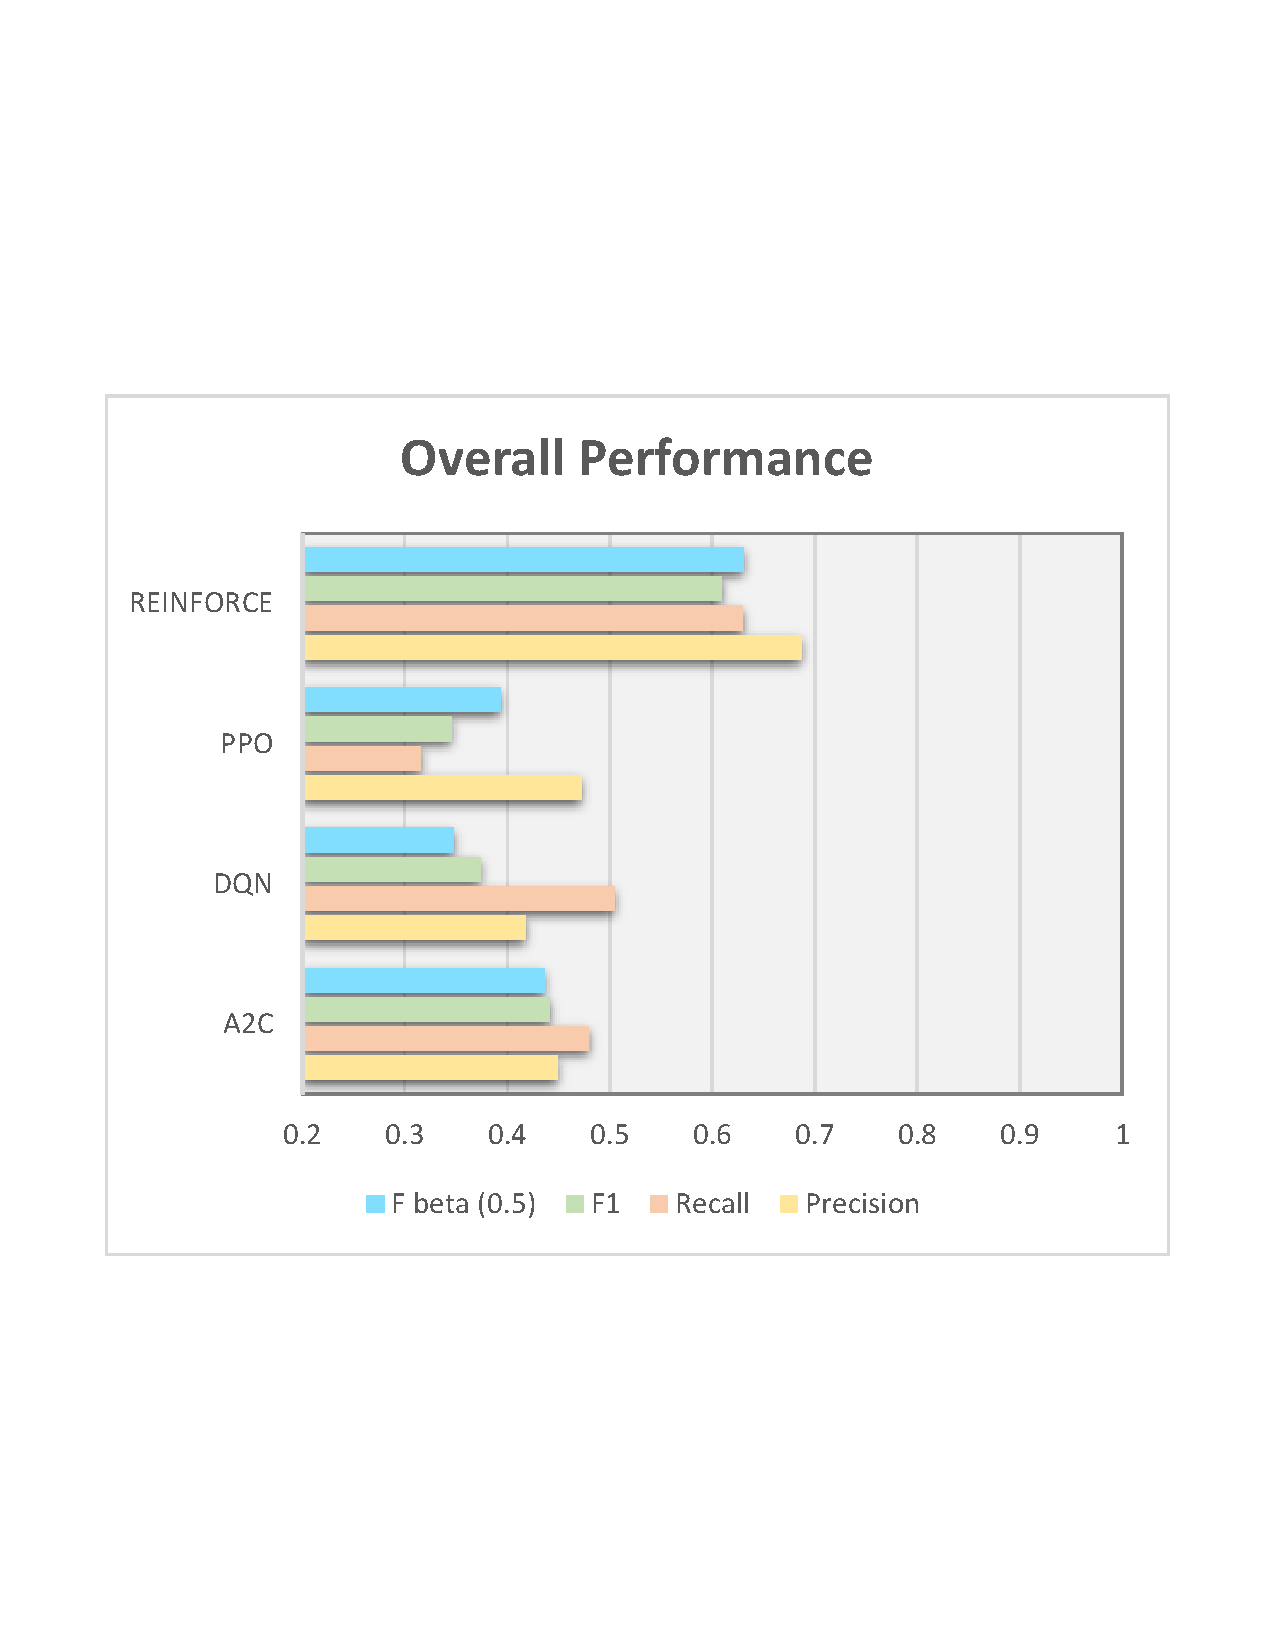
\includegraphics[width=0.6\textwidth, trim={1.5cm 7cm 1cm 7cm}]{images/OverallPlot.pdf}  
	\caption{Overall model performance summary}
	\label{fig:OverallSummary}
\end{figure}
\hlc{At an aggregated level, Table {\ref{tbl:OverallSummary}} along with Fig. {\ref{fig:OverallSummary}}, show that the REINFORCE scores better than the other algorithms, on all four metrics. Tool replacement precision at 0.687, is highest of the four algorithms and better by 0.215 in absolute terms when compared to the next best, PPO. The standard deviation for precision is the lowest at 0.059. On recall, F1 and F-beta (0.5), REINFORCE is better by 0.125, 0.168 and 0.195 compared to the next best.}

\hlc{These metrics were averaged over 10 rounds of training followed by validation. We visualize the behavior of our primary metric F-beta, over the 10 rounds in Fig. {\ref{fig:FbetaOverall}}. The blue line floating above the rest of the algorithms, for all metrics, is that of REINFORCE. The error-bars are also pretty small, indicating lower uncertainty. We notice that the other three algorithms are all centered closely around, 0.4.}
\begin{figure}[h]
 	\centering
 	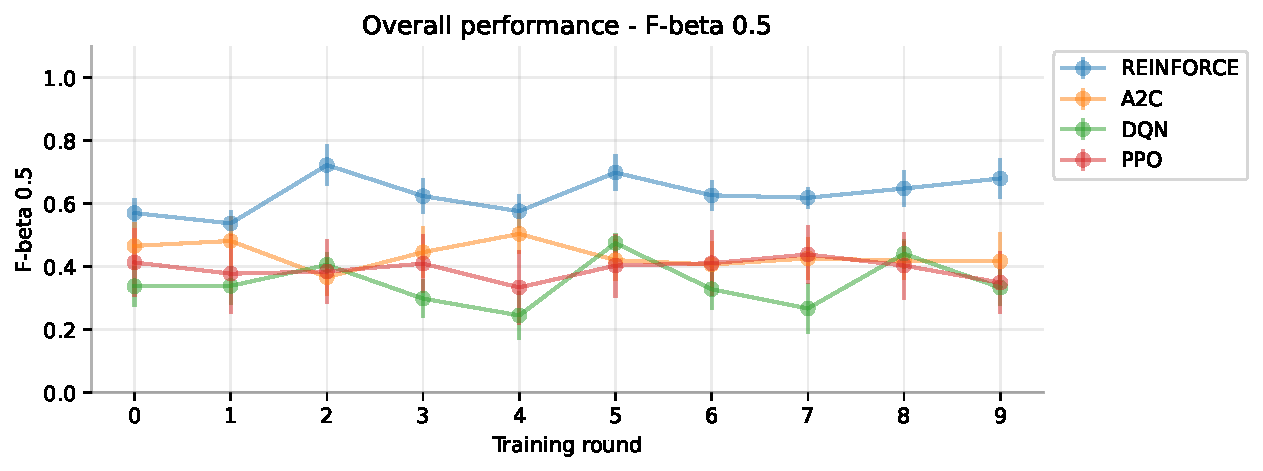
\includegraphics[width=0.9\textwidth]{Overall_F05.pdf}  
 	\caption{Overall performance comparison of the F-beta (0.5) metric, over 10 rounds of training and testing.}
 	\label{fig:FbetaOverall}
\end{figure}

\hlc{We now dig into the detailed metrics Appendix {\ref{apx}} - Table {\ref{tbl:DetailedMetrics}} to better understand the aggregated summary. The largest values are typeset in {\textcolor{dblue}{blue}}. And a quick visual glance shows the dominance of REINFORCE. The notable exceptions are the PHM C01 single-state and no-noise variant where A2C and DQN do better, followed by PHM C01 and PHM C06 univariate-state, low-noise variants where A2C performs better in every aspect and finally the PHM C04 and C06 multivariate variants where A2C again performs better on recall and which in turns drives the F1 score up. Barring these 3 complete cases and 2 cases where A2C recall was better, the REINFORCE performs best in 10 variants and in 2 cases its precision, and therefore F-beta, is highest. This supports the overall performance observed in Table Table {\ref{tbl:OverallSummary}}.}

\subsection{Simulated environment}
\begin{table*}[h]\centering\sffamily
	\rowspace{1.3}
	\begin{tabular}{@{}l rr c rr c rr c rr@{}}
		\arrayrulecolor{black!40}\toprule
		& \multicolumn{2}{c}{Precision} & \phantom{i} & \multicolumn{2}{c}{Recall} & \phantom{i} & \multicolumn{2}{c}{F1-score} & \phantom{i} & \multicolumn{2}{c}{F-beta (0.5)} \\
		\cmidrule{2-3} \cmidrule{5-6} \cmidrule{8-9} \cmidrule{11-12} 
		
		&Mean &SD & &Mean &SD & &Mean &SD& &Mean & SD\\ \midrule
		A2C & 0.416 & 0.120 & &0.385 & 0.073 & & 0.363 & 0.072 & &0.373 &0.082 \\
		DQN & 0.432 & 0.184 & &0.510 & 0.031 & & 0.374 & 0.034 & &0.351 &0.056 \\
		PPO & 0.500 & 0.178 & &0.215 & 0.081 & & 0.285 & 0.099 & &0.370 &0.122 \\
		REINFORCE & \textcolor{dblue}{0.806} & 0.040 & &\textcolor{dblue}{0.915} & 0.038 & & \textcolor{dblue}{0.841} & 0.035 & &\textcolor{dblue}{0.816} &0.037 \\
		
		
		\bottomrule
	\end{tabular}
	\caption{Simulated environments - model performance summary.}
	\label{tbl:SimulatedEnv}
\end{table*}
\begin{figure}[h]
	\centering
	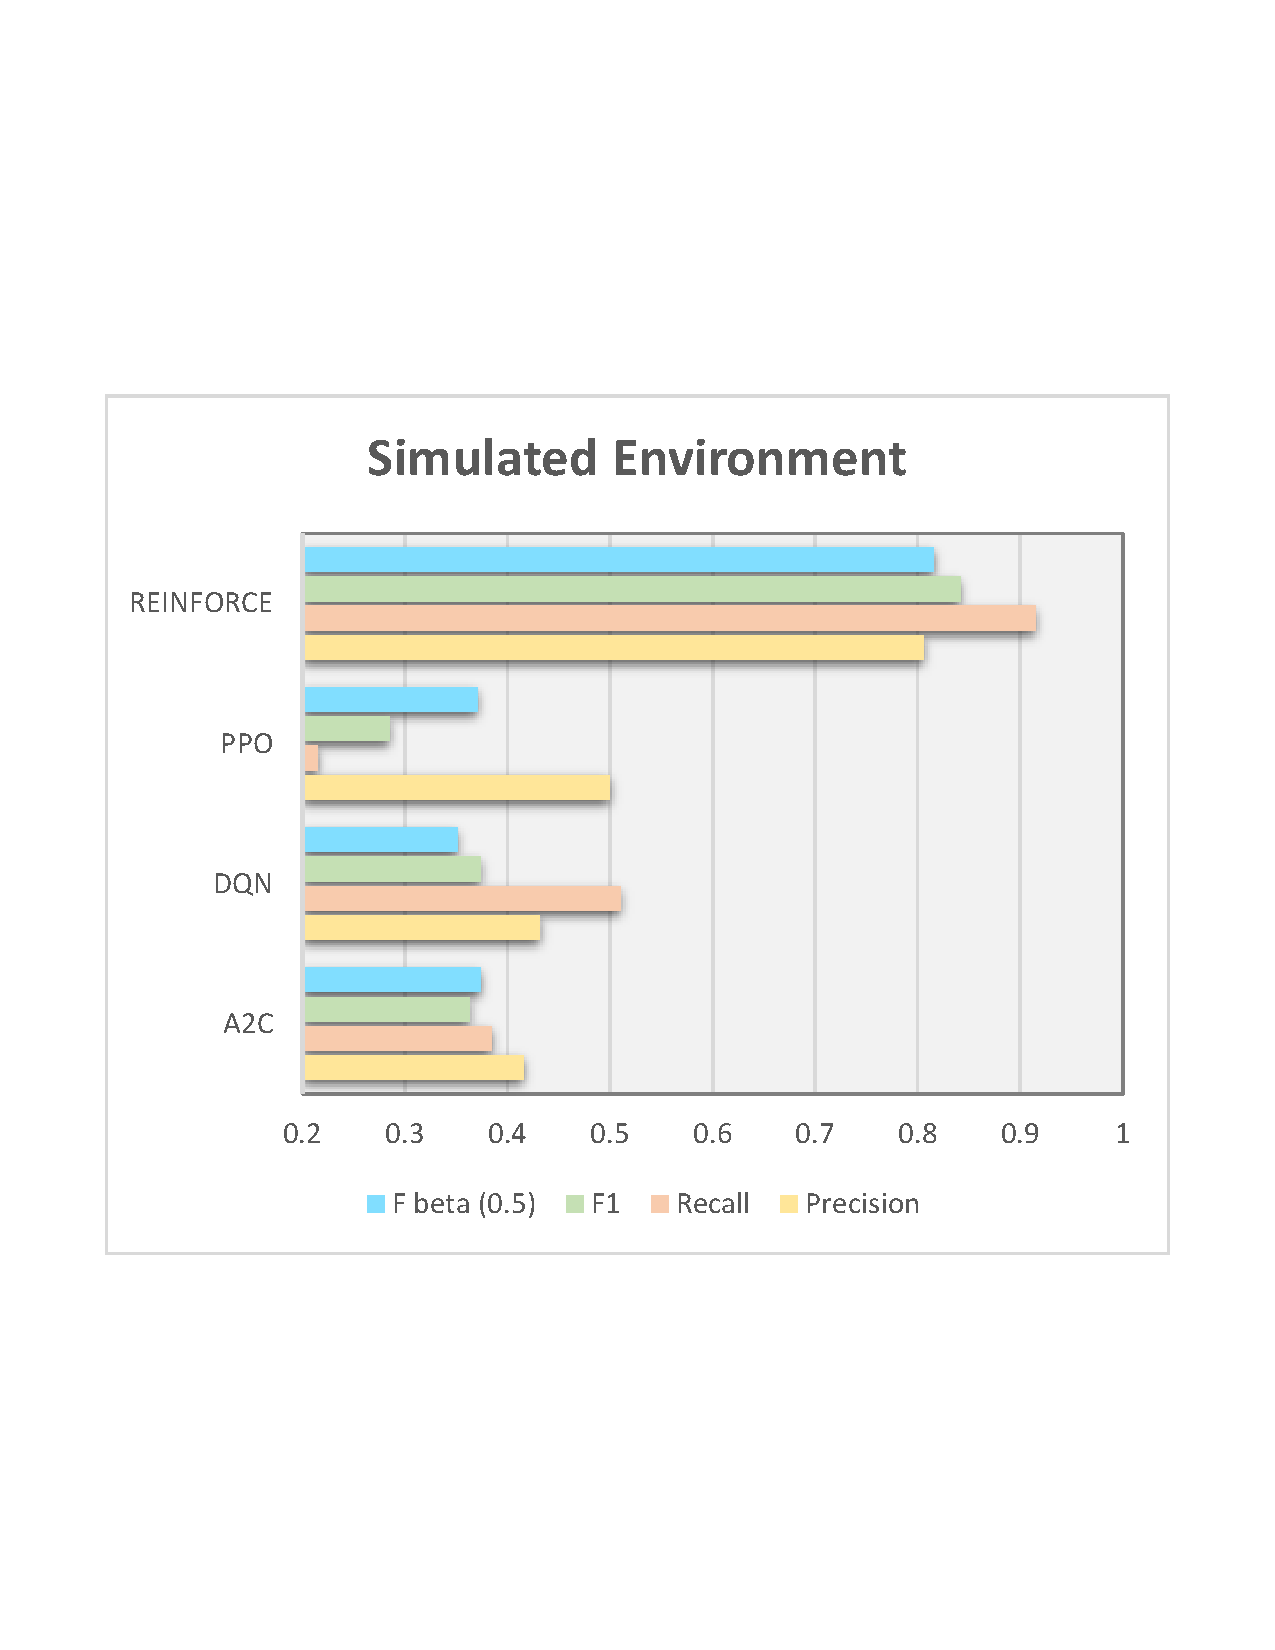
\includegraphics[width=0.6\textwidth, trim={1.5cm 7cm 1cm 7cm}]{images/SimulatedPlot.pdf}  
	\caption{Simulated environments - model performance summary.}
	\label{fig:SimulatedEnv}
\end{figure}
\begin{figure}[h]
	\centering
	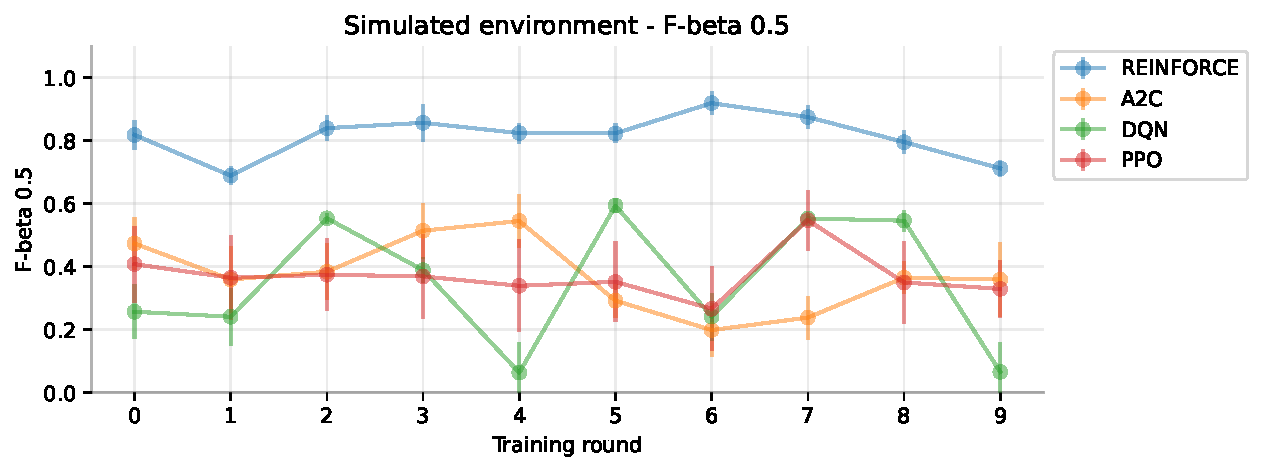
\includegraphics[width=0.9\textwidth]{Simulated_F05.pdf}  
	\caption{Simulated environments - F-beta (0.5) metric, over 10 rounds of training and testing.}
	\label{fig:FbetaSimulated}
\end{figure}

\begin{figure}[h]
	\centering
	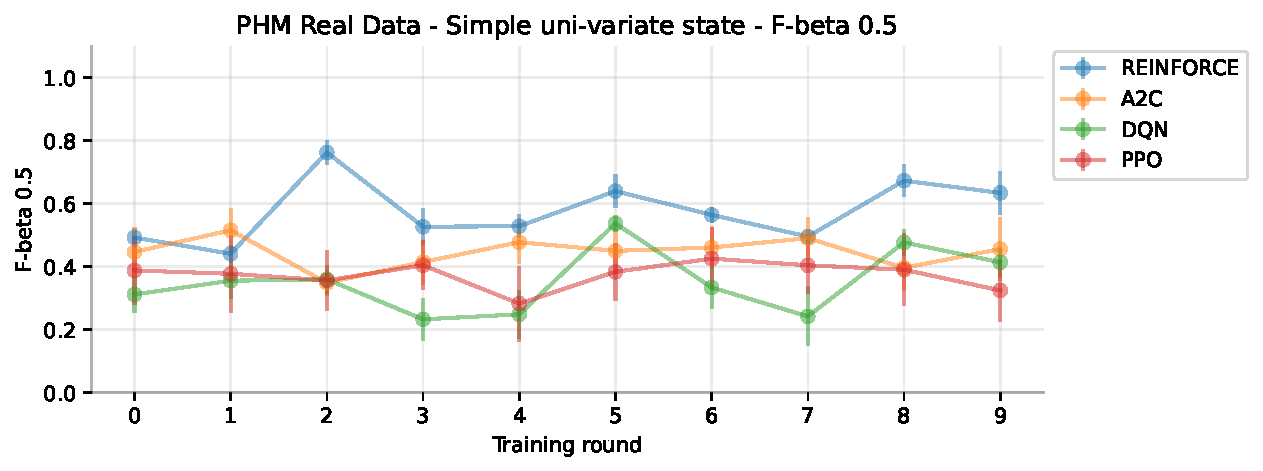
\includegraphics[width=0.9\textwidth]{Singevariable_F05.pdf}  
	\caption{Univariate simple state environments - F-beta (0.5) metric, over 10 rounds of training and testing.}
	\label{fig:FbetaPHMSS}
\end{figure}

\begin{figure}[h]
	\centering
	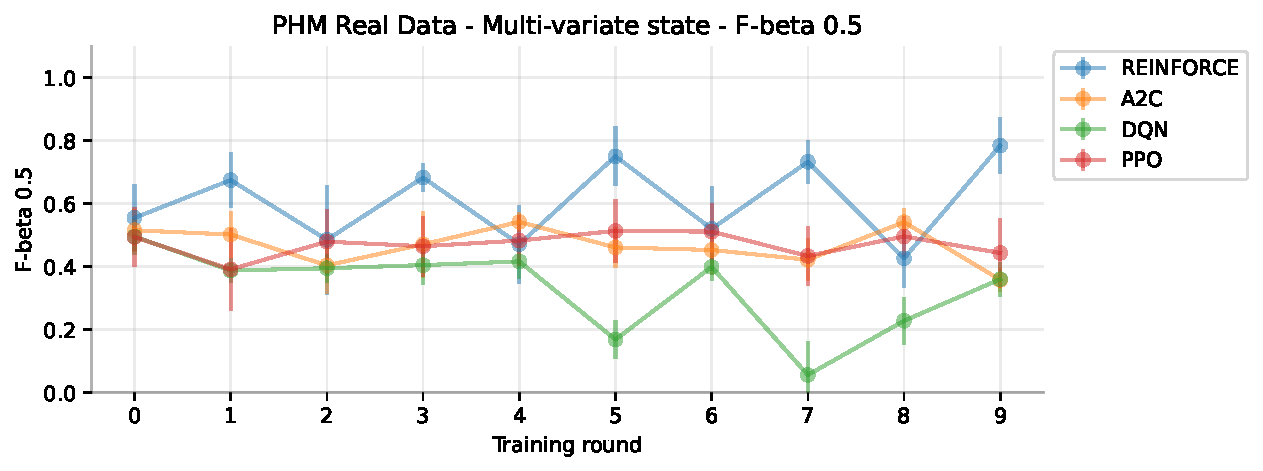
\includegraphics[width=0.9\textwidth]{Multivariate_F05.pdf}  
	\caption{Multivariate complex state environments - F-beta (0.5) metric, over 10 rounds of training and testing.}
	\label{fig:FbetaPHMMS}
\end{figure}

The simulated tool-wear environment is relatively the simplest for the agent to learn. We added two levels of noise and chance of breakdown and averaged the performance over the three variants, Table \ref{tbl:SimulatedEnv}. The REINFORCE performs the best and in absolute terms it is better than the next best advanced algorithm by very high margins: precision by 0.306, recall by 0.405, F1 by 0.468 and F-beta (0.5) by 0.442, with standard deviation lower or marginally higher than others. Plot Fig. \ref{fig:tr-sim-env} shows DQN having very high fluctuations, occasionally showing recalls at the REINFORCE levels (rounds 2 and 8).

\subsection{Real data - simple univariate environment}
\begin{table*}[h]\centering
	\sffamily
	\rowspace{1.3}
	\begin{tabular}{@{}l rr c rr c rr c rr@{}}
		\arrayrulecolor{black!40}\toprule
		& \multicolumn{2}{c}{Precision} & \phantom{i} & \multicolumn{2}{c}{Recall} & \phantom{i} & \multicolumn{2}{c}{F1-score} & \phantom{i} & \multicolumn{2}{c}{F-beta (0.5)} \\
		\cmidrule{2-3} \cmidrule{5-6} \cmidrule{8-9} \cmidrule{11-12} 
		
		&Mean &SD & &Mean &SD & &Mean &SD& &Mean & SD\\ \midrule
		A2C & 0.447 & 0.077 & &0.477 & 0.091 & & 0.452 & 0.072 & &0.446 &0.070 \\
		DQN & 0.419 & 0.179 & &0.507 & 0.032 & & 0.379 & 0.036 & &0.352 &0.057 \\
		PPO & 0.450 & 0.146 & &0.314 & 0.082 & & 0.333 & 0.087 & &0.374 &0.102 \\
		REINFORCE & \textcolor{dblue}{0.605} & 0.046 & &\textcolor{dblue}{0.603} & 0.046 & & \textcolor{dblue}{0.570} & 0.041 & &\textcolor{dblue}{0.576} &0.040 \\
		
		\bottomrule
	\end{tabular}
	\caption{Model performance summary - averaged over PHM-2010 environments with simple single-variable environment.}
	\label{tbl:PHMSS}
\end{table*}
\begin{figure}[h]
	\centering
	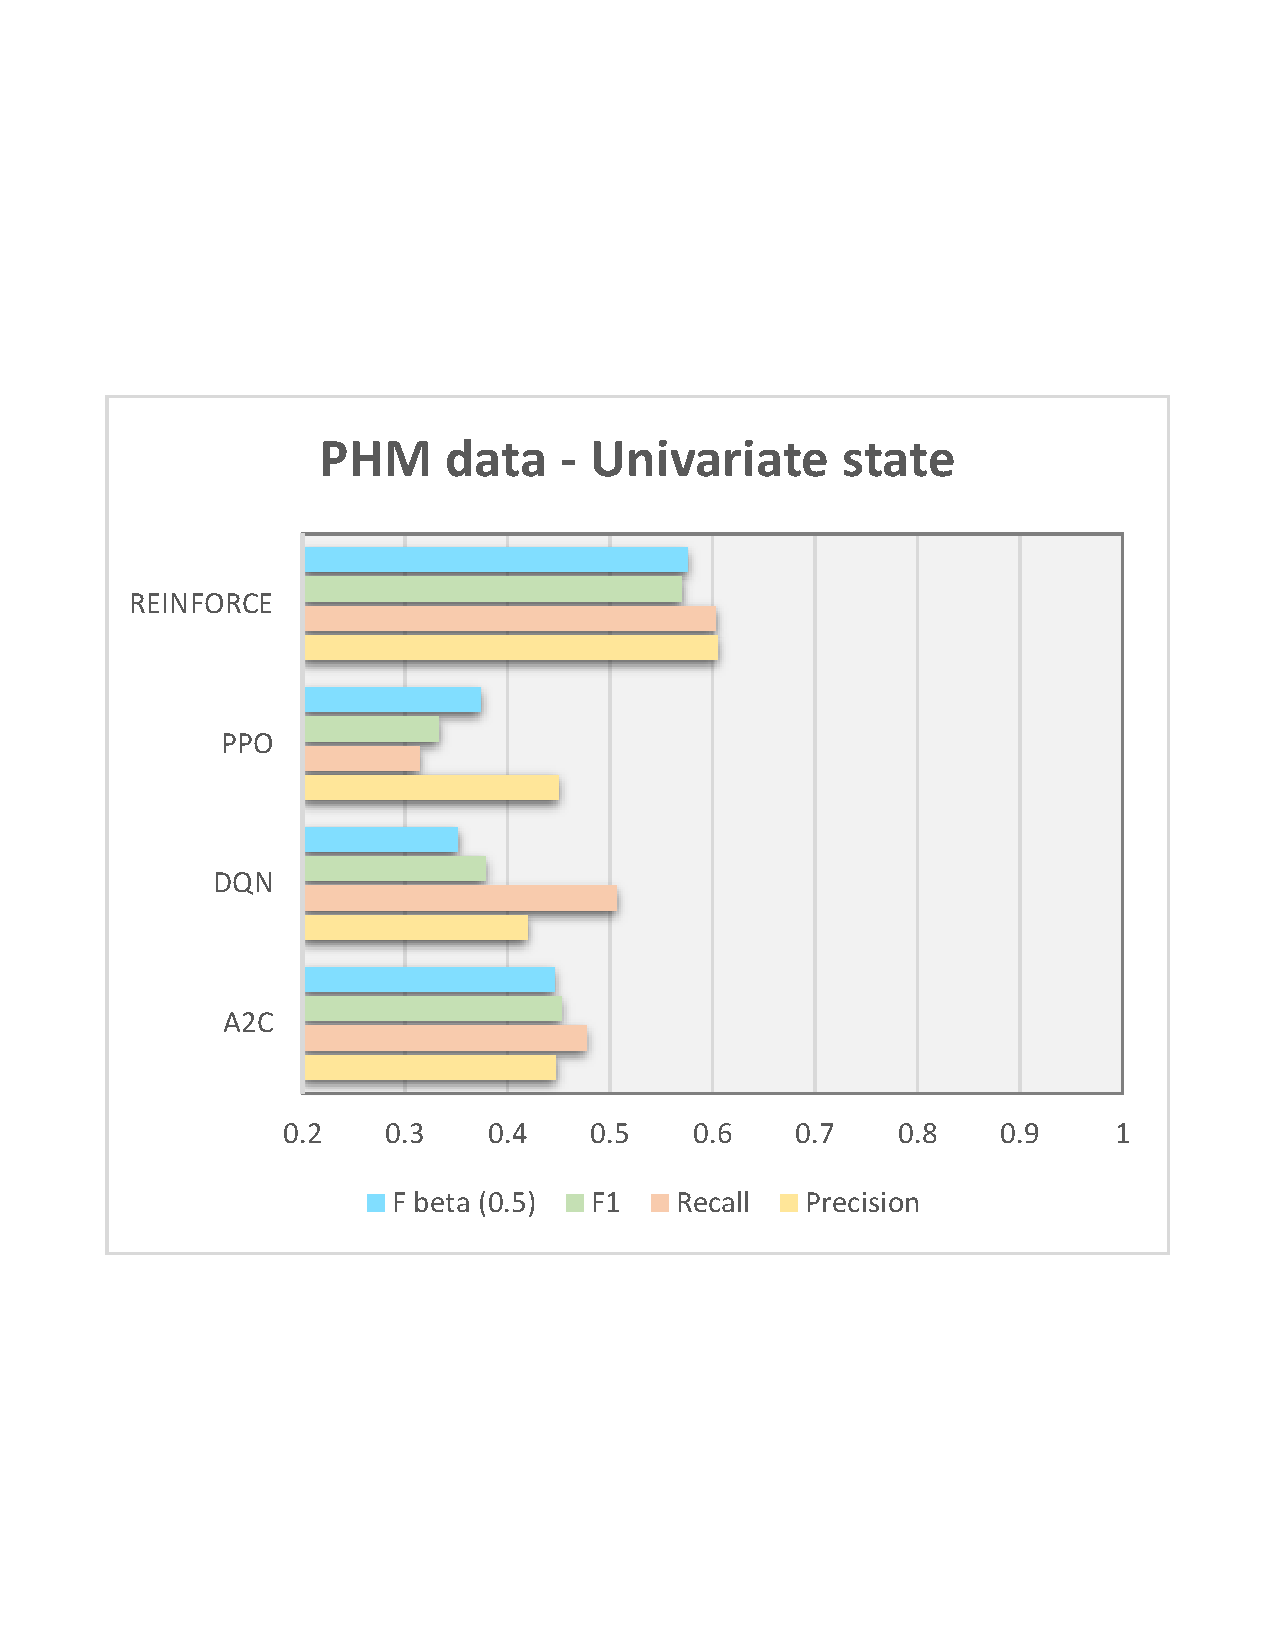
\includegraphics[width=0.6\textwidth, trim={1.5cm 7cm 1cm 7cm}]{images/PHMSSPlot.pdf}  
	\caption{PHM real data - Model performance summary for the simple single-variable environment.}
	\label{fig:PHMSS}
\end{figure}
Real data offers a more challenging environment. Despite this, in Table \ref{tbl:PHMSS}, we notice that REINFORCE  still performs better than the other algorithms. The margins are understandably lower: precision by 0.155, recall by 0.097, F1 by 0.117 and F-beta (0.5) by 0.130. Fig. \ref{fig:tr-ss-env} shows the plots for the simple univariate state. While the REINFORCE precision is higher for most rounds, the recall seems to be occasionally surpassed slightly by DQN's (1, 8 and 9) and by a larger margin once (5).

\subsection{Real data - complex multivariate state}
\begin{table*}[!htb]\centering
	\sffamily
	\rowspace{1.3}
	\begin{tabular}{@{}l rr c rr c rr c rr@{}}
		\arrayrulecolor{black!40}\toprule
		& \multicolumn{2}{c}{Precision} & \phantom{i} & \multicolumn{2}{c}{Recall} & \phantom{i} & \multicolumn{2}{c}{F1-score} & \phantom{i} & \multicolumn{2}{c}{F-beta (0.5)} \\
		\cmidrule{2-3} \cmidrule{5-6} \cmidrule{8-9} \cmidrule{11-12} 
		
		&Mean &SD & &Mean &SD & &Mean &SD& &Mean & SD\\ \midrule
		A2C & 0.487 & 0.086 & &\textcolor{dblue}{0.582} & 0.075 & & 0.488 & 0.063 & &0.467 &0.065 \\
		DQN & 0.399 & 0.204 & &0.491 & 0.032 & & 0.361 & 0.035 & &0.332 &0.060 \\
		PPO & 0.512 & 0.107 & &0.422 & 0.107 & & 0.441 & 0.096 & &0.472 &0.096 \\
		REINFORCE & \textcolor{dblue}{0.813} & 0.119 & &0.421 & 0.079 & & \textcolor{dblue}{0.495} & 0.090 & &\textcolor{dblue}{0.609} &0.101 \\
		\bottomrule
	\end{tabular}
	\caption{Model performance summary - averaged over PHM-2010 environments with complex multivariate environment.}
	\label{tbl:PHMMS}
\end{table*}
\begin{figure}[h]
	\centering
	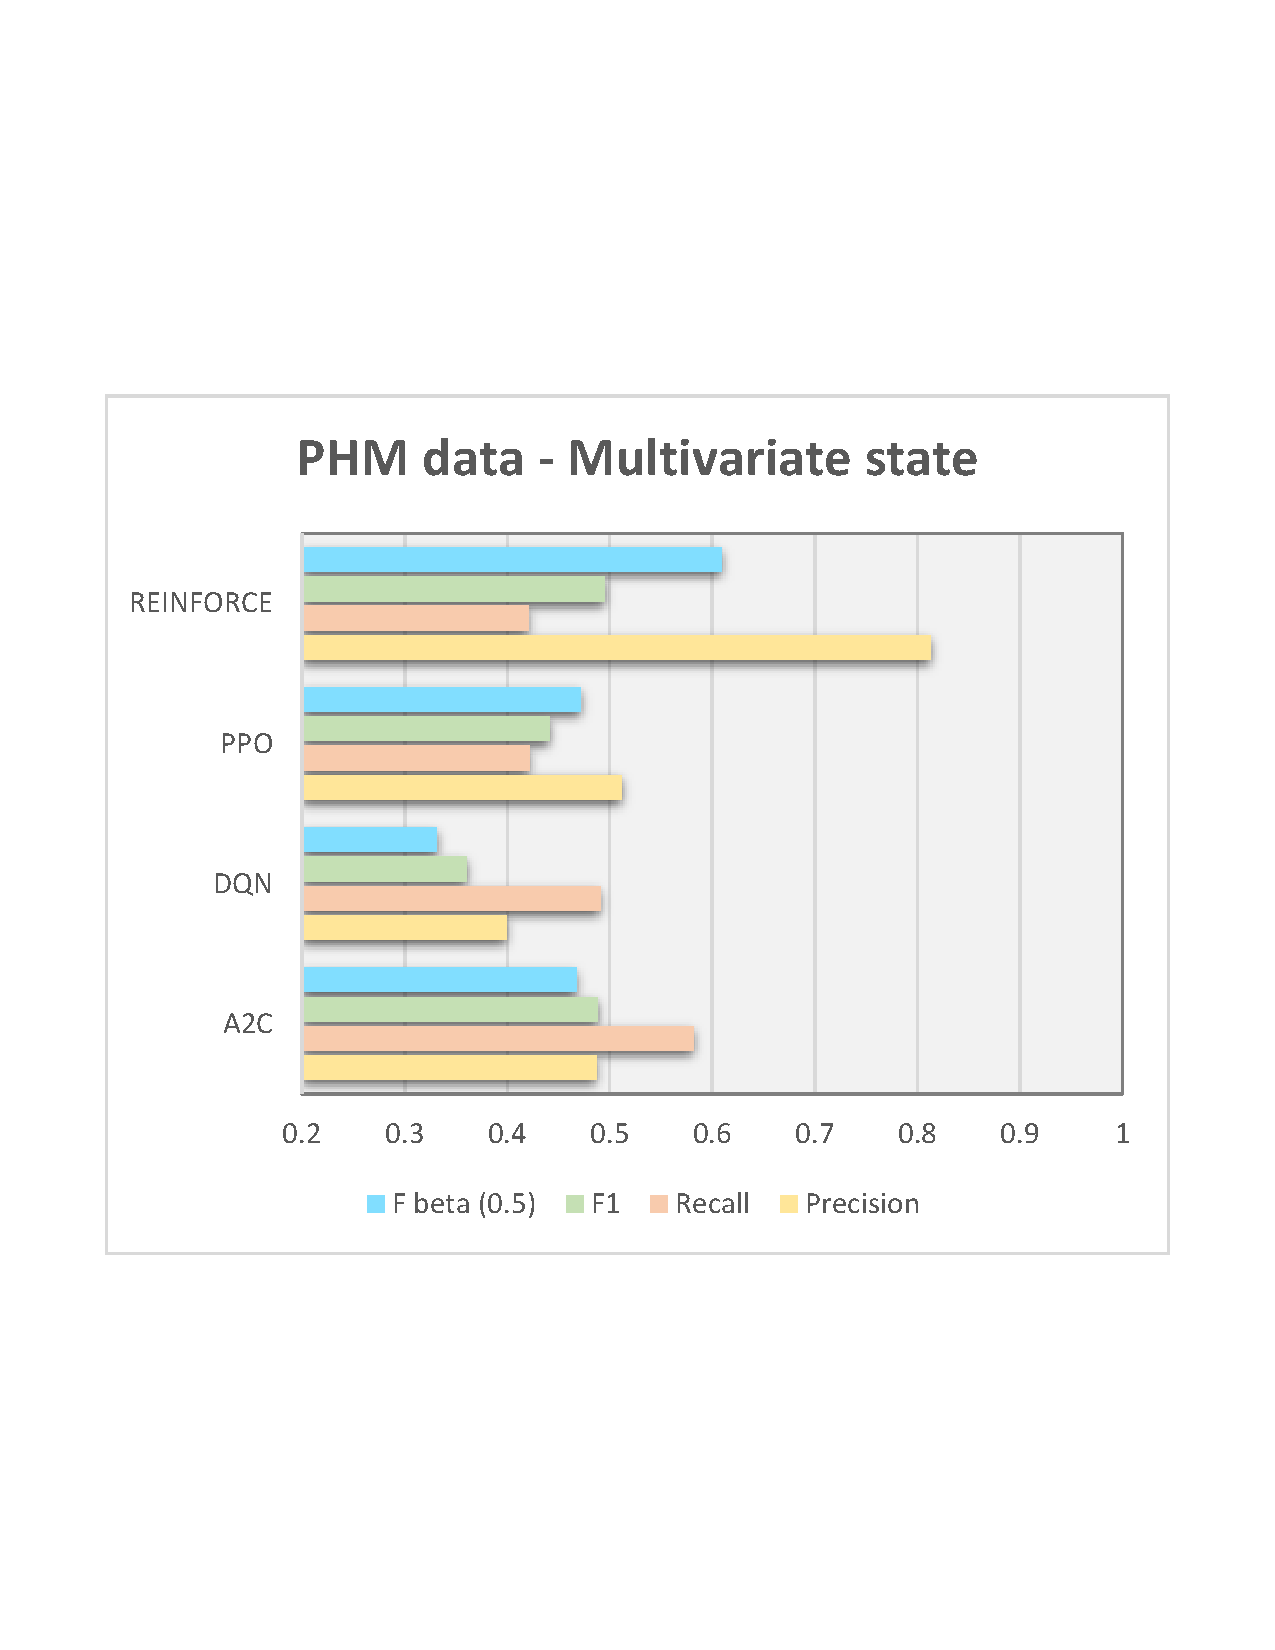
\includegraphics[width=0.6\textwidth, trim={1.5cm 7cm 1cm 7cm}]{images/PHMMSPlot.pdf}  
	\caption{PHM real data - Model performance summary for the complex multivariate environment.}
	\label{fig:PHMMS}
\end{figure}
This environment offers the highest difficulty. We use real data, from \textit{multiple} sensors. As with other scenarios, we used untuned, default settings of all algorithms. In Table \ref{tbl:PHMSS}, we see that the REINFORCE has the poorest recall at 0.421, however it demonstrates a surprisingly high tool replacement precision at 0.813, which dr ives the F1 and F-beta to the top of the table. The plot, Fig. \ref{fig:tr-ms-env} shows REINFORCE's high precision behavior. However, it is important to note that the error-bars are occasionally larger (rounds 0, 2, 4 and 6). The recall seemed higher at some points but lower half the times. The F1 appears to in range of all the other algorithms.

\subsection{Super models}
Finally, we look at performance of ``select'' models. Logically, one would choose the best model from a set of 10 trained models. Selecting models that produce the highest F1 with a minimum criteria for precision and recall allowed us to evaluate performance of ``super-models'' for each algorithm. In Table \ref{tbl:SuperModelsDetailedMetrics}, the REINFORCE performs better than the other three algorithms by a huge margin, for 14 of the 15 variants. For the PHM C06, univariate environment, the DQN performs the best, with extremely high metrics throughout and an F1 of 0.969 to 0.831 of REINFORCE.

As an overall average performance, Table \ref{tbl:supermodels} demonstrates the remarkable performance of the simple REINFORCE algorithm. It does show a lower recall when compared to the DQN, however it is a much more \textit{balanced} model on an overall basis.
\begin{table*}[h]\centering
	\sffamily
	\rowspace{1.3}
	\begin{tabular}{@{}l rr c rr c rr c rr@{}}
		\arrayrulecolor{black!40}\toprule
		& \multicolumn{2}{c}{Precision} & \phantom{i} & \multicolumn{2}{c}{Recall} & \phantom{i} & \multicolumn{2}{c}{F1-score} & \phantom{i} & \multicolumn{2}{c}{F-beta (0.5)} \\
		\cmidrule{2-3} \cmidrule{5-6} \cmidrule{8-9} \cmidrule{11-12} 
		
		&Mean &SD & &Mean &SD & &Mean &SD& &Mean & SD\\ \midrule
		A2C & 0.520 & 0.031 & &0.859 & 0.053 & & 0.639 & 0.036 & &0.560 &0.032 \\
		DQN & 0.651 & 0.022 & &0.937 & 0.031 & & 0.740 & 0.022 & &0.678 &0.021 \\
		PPO & 0.558 & 0.076 & &0.643 & 0.097 & & 0.580 & 0.079 & &0.562 &0.075 \\
		REINFORCE & \textcolor{dblue}{0.884} & 0.042 & &\textcolor{dblue}{0.884} & 0.042 & & \textcolor{dblue}{0.873} & 0.034 & &\textcolor{dblue}{0.876} &0.036 \\
		\bottomrule
	\end{tabular}
	\caption{Super models: Best of 10 rounds; performance averaged over all 15 environments.}
	\label{tbl:supermodels}
\end{table*}
\begin{figure}[!htbp]
	\centering
	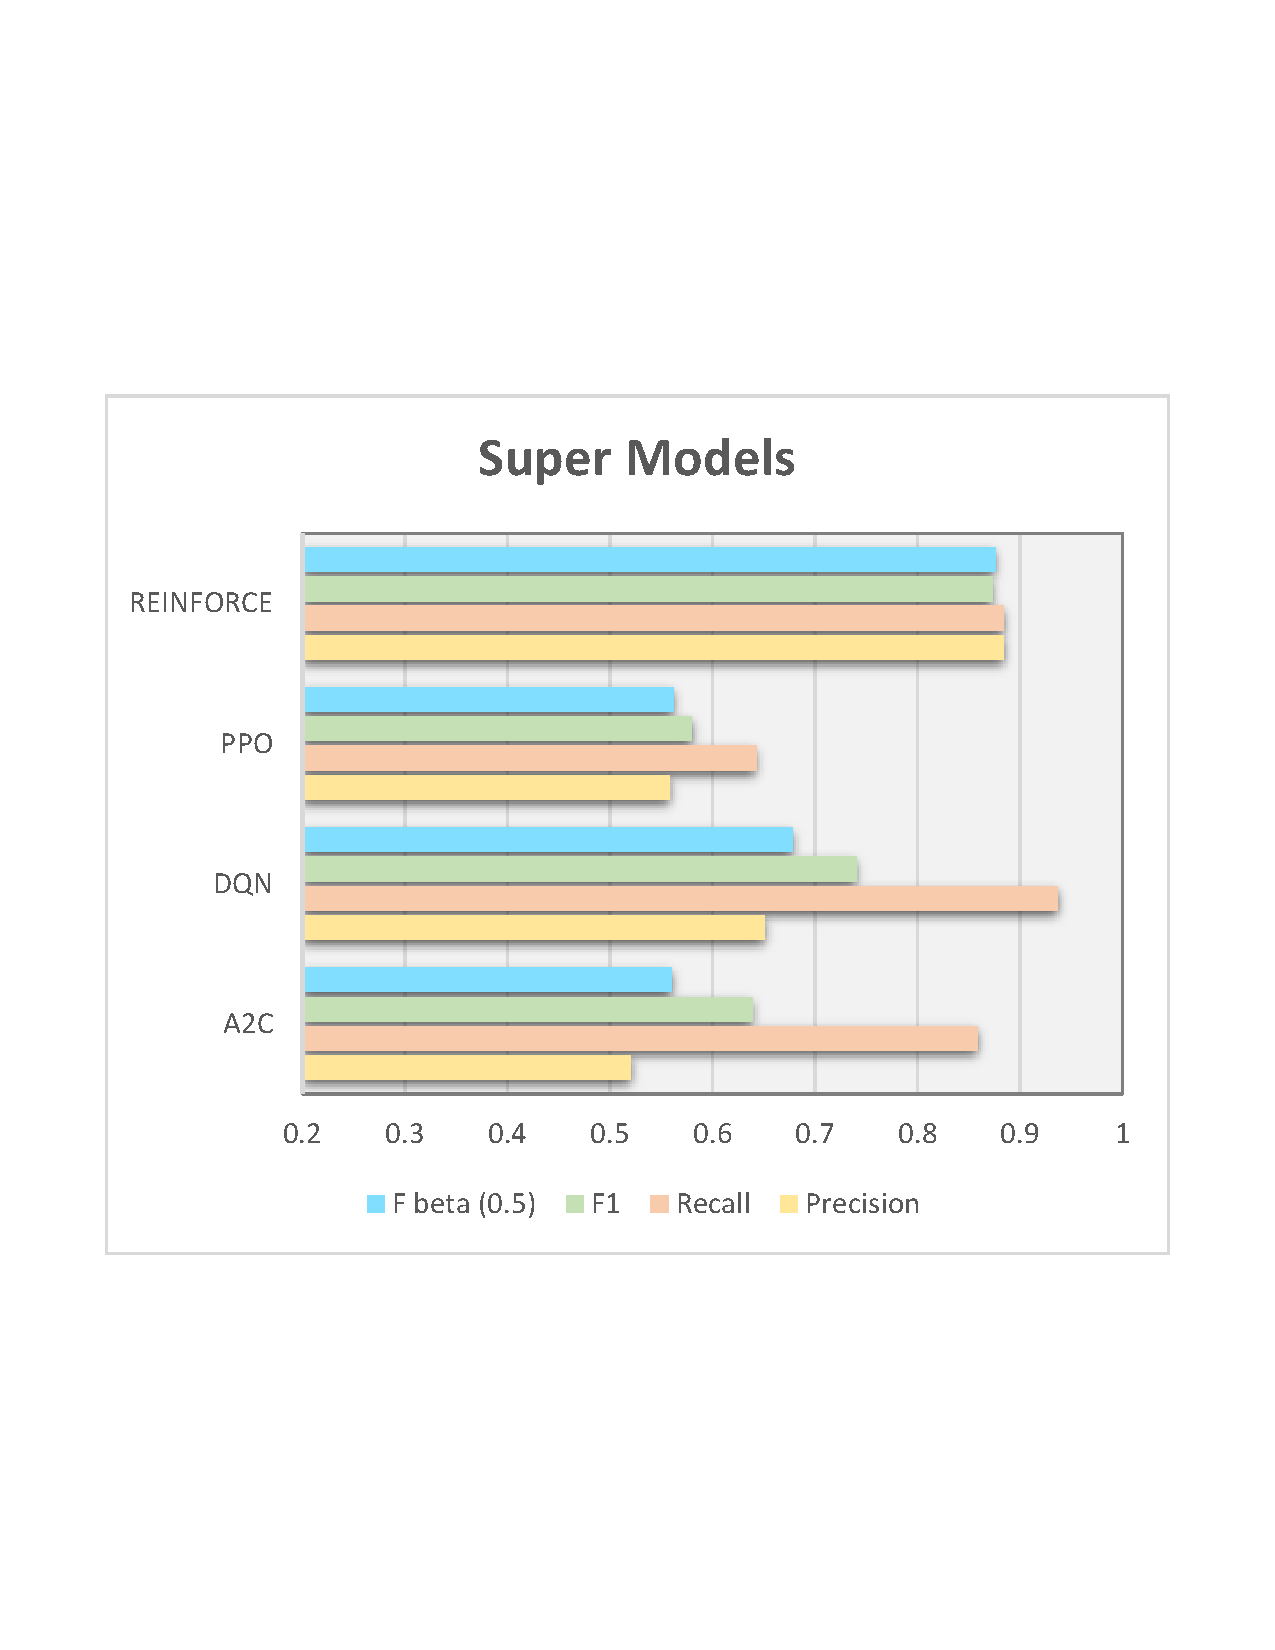
\includegraphics[width=0.6\textwidth, trim={1.5cm 7cm 1cm 7cm}]{images/SuperModelsPlot.pdf}  
	\caption{Super models: Best of 10 rounds; performance averaged over all 15 environments.}
	\label{fig:supermodels}
\end{figure}

\subsection{Hypothesis testing}
We undertake a statistical analysis of the results, postulated by the hypothesis (\ref{eq:Hypothesis}). Table \ref{tbl:ttest} shows the result of a one-sided, two-sample t-test, conducted for a significance level $\alpha=0.05$. Sample size of the test are mentioned against each category\footnote{What does a single data point indicate?: Consider the ``Simulated'' category -- 10 training rounds $\times$ 10 test rounds $\times$ 3 noise settings = 300 sample points. Note that a single test round is conducted with 40 randomly sampled wear datapoints and therefore 300 samples = 300 $\times$40 i.e. 12,000 samples of wear data. Similarly, for the real-data univariate state: 3 datasets $\times$ 10 training rounds $\times$ 10 test rounds $\times$3 noise settings = 900 sample points.}.
\begin{equation}
	\left.\begin{aligned}
		H_0 & : \mu_{RF} - \mu_{AA} = 0,\;\; \\
		H_a & : \mu_{RF} - \mu_{AA} > 0, \;\;
	\end{aligned}
	\right\}
	\qquad \forall \;\; \text{$AA \in[A2C, DQN, PPO]$}
	\label{eq:Hypothesis}
\end{equation}
We see that the p-values are extremely low and test statistic positive, for all cases except for the \textit{recall} in the PHM multivariate state case. We can thus reject $H_0$.

\begin{table*}[hbt!]\centering
	\sffamily
	\rowspace{1.3}
	\begin{tabular}{@{}l c rrr c l rrr @{}}
		\arrayrulecolor{black!40}\toprule
		
		&& \multicolumn{3}{c}{\textbf{p Value}} & \phantom{i} & & \multicolumn{3}{c}{\textbf{t Statistic}} \\
		\cmidrule{3-5} \cmidrule{8-10} 
		
		Metric && \small {RF $\underset{H_0}{\overset{H_a}{\geqq}}$A2C} &\small {RF $\underset{H_0}{\overset{H_a}{\geqq}}$DQN} &\small {RF $\underset{H_0}{\overset{H_a}{\geqq}}$PPO} & & & \small {RF $\underset{H_0}{\overset{H_a}{\geqq}}$A2C} &\small {RF $\underset{H_0}{\overset{H_a}{\geqq}}$DQN} &\small {RF $\underset{H_0}{\overset{H_a}{\geqq}}$PPO} \\ \midrule 
		\multicolumn{10}{@{}l}{\textbf{Overall} (1500 samples)} \\[6pt]
		Precision & &4.31E-126 &2.17E-109 &2.81E-106 & & &25.071 &23.170 &22.804\\
		Recall & &4.20E-35 &3.37E-16 &4.36E-150 & & &12.522 &8.206 &27.650\\
		F1 score & &1.99E-64 &1.46E-88 &5.29E-155 & & &17.364 &20.634 &28.160\\[6pt]\midrule
		
		\multicolumn{10}{@{}l}{\textbf{Simulated environment} (300 samples)}\\[6pt]
		Precision & &3.20E-98 &1.69E-63 &2.65E-81 & & &25.611 &19.032 &22.427\\
		Recall & &8.12E-104 &2.56E-41 &1.57E-264 & & &26.665 &14.558 &62.541\\
		F1 score & &9.60E-134 &8.56E-99 &2.96E-242 & & &32.402 &25.719 &56.575\\[6pt] \midrule
		
		\multicolumn{10}{@{}l}{\textbf{PHM Real data - Simple univariate state} (900 samples)} \\[6pt]
		Precision & &2.27E-32 &7.29E-31 &9.95E-31 & & &12.082 &11.770 &11.742\\
		Recall & &1.27E-16 &1.55E-06 &8.19E-71 & & &8.357 &4.821 &18.607\\
		F1 score & &1.94E-19 &4.67E-34 &2.19E-67 & & &9.121 &12.423 &18.098\\ [6pt]\midrule
		
		\multicolumn{10}{@{}l}{\textbf{PHM Real data - Complex multivariate state} (300 samples)}\\[6pt]
		Precision & &1.64E-60 &3.34E-54 &7.88E-59 & & &18.451 &17.207 &18.122\\
		Recall & &2.69E-10 &2.69E-02 &9.68E-01 & & &-6.425 &-2.219 &-0.041\\
		F1 score & &7.27E-01 &1.44E-08 &1.35E-03 & & &0.349 &5.748 &3.220\\
		\bottomrule
	\end{tabular}
	\caption{Statistical test: One-sided two-sample t-tests. $H_0: \mu_{RF}-\mu_{AA}=0; H_a: \mu_{RF}-\mu_{AA} > 0$, where $AA$is one of A2C, DQN or PPO}
	\label{tbl:ttest}
\end{table*}

\subsection{Training times}
Our final set of results are related to the training time required for each algorithm. The na\"ive REINFORCE algorithm is extremely slow, with a very high variance in training time, as seen in Fig. \ref{fig:tr-time}.
\begin{figure}[ht]
	\centering
	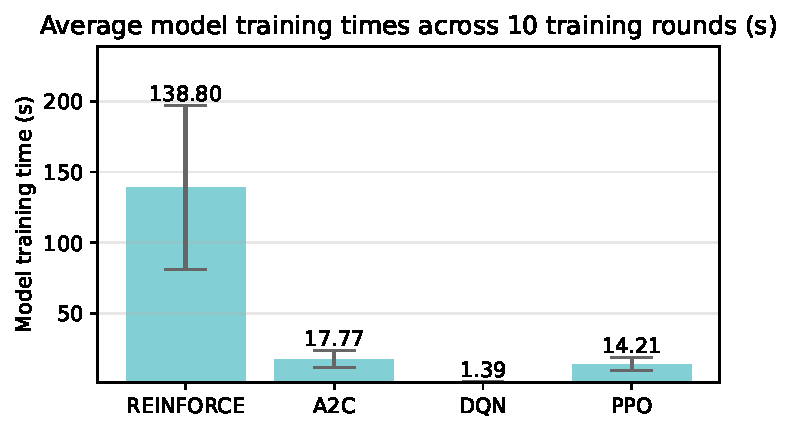
\includegraphics[width=0.6\linewidth]{Model_training_time.pdf}  
	\caption{Training time, averaged over 10 rounds and all 15 variants.}
	\label{fig:tr-time}
\end{figure}

\section{Discussion}\label{sec:Discussion}
The inventor of the REINFORCE algorithm, in his original paper \cite{REINFORCE-williams1992}, mentions the inability to predict the convergent and asymptotic properties of REINFORCE algorithms using analytical means. The author mentions that \textit{simulation studies} are the primary source of understanding its behavior. 27 years later, \cite{peck2019} notes that rigorous convergence proofs are \textit{not} available for many algorithms based on REINFORCE and in their paper provide an intuition for convergence properties. This supports the extensive experimental studies on REINFORCE performed by \cite{zhang2021sample, zhang2021convergence, peck2019, duan2016benchmarking} as well our empirical research.

Both \cite{duan2016benchmarking} and \cite{zhang2021convergence} studied the behavior on multiple OpenAI Gym environments, while \cite{peck2019} provide empirical results for MuJuCo environments. \cite{duan2016benchmarking} observe that, despite its simplicity it is an effective algorithm in optimizing policies based on deep neural networks. On the other hand, their empirical study concluded that REINFORCE is occasionally trapped in premature convergence to local optima. REINFORCE suffers from high variance \citep{peck2019} and converges very slowly when it does. High variance implies that a large sample of environment interactions are needed to obtain a reasonable approximation of the actual gradient. 

\cite{zhang2021sample} provide the first known global convergence and sample efficiency results for the REINFORCE algorithm. Their study involved controlling the number of ``bad'' episodes as well as applying a ``doubling'' trick for studying the global convergence. Interestingly our training rounds resulted in multiple situations of ``zero'' performance (``bad'' episodes) for REINFORCE (18 instances) as also for Stable-Baseline's A2C implementation (12 instances); DQN and PPO did not show any occurrences. %, Table \ref{tbl:BadEpisodes}. 

There could be two possible reasons for the positive performance demonstrated by REINFORCE. We used ReLU (rectified linear unit) as the activation function, while the other three algorithms used hyperbolic tangent (Tanh). \cite{henderson2018deep} studied four policy-gradient methods, including the PPO and TRPO, and observed that ReLU activation perform best. \cite{duan2016benchmarking} observed that \textit{even} with a small learning rate REINFORCE sometimes resulted in large changes to policy distribution, which possibly explains the fast convergence to local optima. On the other hand we used a larger learning rate (almost 50:1) and this could have assisted in reaching global optimas when it did. %An additional thread that needs exploration is ``over-fitting and saturation'' as studied by \cite{song2019} for model-free RL. \cite{hardt2016} theoretically prove that stochastic gradient methods when trained using fewer iterations, have vanishing generalization errors. Their experiments conclude that shortened training time by itself, sufficiently prevents over-fitting. In our experiments we used 800 or 1000 episodes for REINFORCE versus 10,000 for A2C, DQN and PPO. 

While there is no doubt that this REINFORCE na\"ive implementation will be unstable and occasionally produce learning patterns that are stuck in local optimas and demonstrate premature convergence, our empirical studies indicate that it did perform well for this problem and at the least deserves further research.
%\begin{table*}					
%	\sffamily				
%	\rowspace{1.3}				
%	\begin{tabular}{@{}r l rr} \arrayrulecolor{black!40}\toprule 
%		& Environment variant & A2C & REINFORCE\\ \midrule				
%		& \multicolumn{3}{l}{\textbf{Simulated}}\\		
%		1 & Simulated - No noise  & 2	& \\
%		2 & Simulated - Low noise & & \\	
%		3 &	Simulated  - High noise & 1 &\\ \midrule
%		\rule{0pt}{1.5\normalbaselineskip}			
%		& \multicolumn{3}{l}{\textbf{Real data -- simple univariate}} \\		
%		4 &	PHM C01 SS (simple, univariate) - No noise &	&	5 \\
%		5 &	PHM C01 SS (simple, univariate) - Low noise &	&	4 \\
%		6 &	PHM C01 SS (simple, univariate) - High noise &	3 &	1 \\ \hdashline
%		
%		7 & PHM C04 SS (simple, univariate) - No noise & & \\		
%		8 &	PHM C04 SS (simple, univariate) - Low noise & 2 &\\
%		9 &	PHM C04 SS (simple, univariate) - High noise & & \\	\hdashline
%		
%		10 & PHM C06 SS (simple, univariate) - No noise & & 1 \\
%		11 & PHM C06 SS (simple, univariate) - Low noise & & 7 \\
%		12 & PHM C06 SS (simple, univariate - High noise & 3 & \\ \midrule
%		\rule{0pt}{1.5\normalbaselineskip}			
%		& \multicolumn{3}{l}{\textbf{Real data -- complex multivariate}} \\		
%		13 & PHM C01 MS (complex, multivariate) - No noise & 1 &\\
%		14 & PHM C04 MS (complex, multivariate) - Low noise & &\\		
%		15 & PHM C06 MS (complex, multivariate) - High noise & & \\ \bottomrule	
%	\end{tabular}				
%	\caption{``Bad'' episodes - Number of training rounds across the fifteen environments where no learning occured. DQN and PPO did not show any occurences.}				
%	\label{tbl:BadEpisodes}				
%\end{table*}					

\textbf{On the evaluation criteria:} It must be noted that the classification metrics we used assume that the human preventive maintenance policy, based on experience, is ideal. In practice this might not always be the case. The RL agent is trained to replace the tool optimally i.e. maximize use before reaching the threshold wear, and replace only when necessary so as to maintain lowest possible cost of replacement. In our dataset we assume the threshold to be ideally set and base the ``human'' action against that, rather than a real human action, which incidentally is not available for the PHM dataset anyway.

%% $$$IMPORTANT
%\textbf{On precision and recall control}: High precision implies lower $FP$i.e. false replacement action reduced i.e. unnecessary tool replacements reduced. Tool life maximized, down time minimized, production disruption minimized.  High recall implies lower $FN$, i.e. false declaration of ``normal  state'' reduced, so true normal state detection increased.

%\textbf{On the reward function:} Default value for $R3$was $-40$. A higher penalty for tool replacement improves recall, while a lower penalty improved precision.
 
%- Transition function \citep{graesser2019}: pg333 "Transition function  - also known as model. can be learnt or programmed programmable rules are common and lead to increasing complexity. \textcolor{red}{***} We use a hybrid model - partly learnt and partly programmed": \textbf{Noise and breakdown}\\
%% $$$IMPORTANT

\section{Conclusion}\label{sec:Conclusion}
The REINFORCE is a simple algorithm and our na\"ive implementation can be improved drastically, for example with the implementation of a baseline to reduce variance. We evaluated the REINFORCE along with industry grade implementations of more advanced algorithms, DQN, A2C and PPO, over 15 environment variants (simulated and real data). Despite its simplicity, known variance and convergence issues, it performed surprisingly well, as observed through numerical results, plots and statistical tests. 

Implementing robust RL algorithms is complex and \cite{SB3-paper} mention how small implementation details can significantly impact performance that is often greater than the difference between the algorithms themselves. We hope our research will contribute to empirical evidence in the study of REINFORCE and therefore contribute in an infinitesimal way to enable AutoML for the field of predictive maintenance using RL. %conducted on non-OpenAI-Gym environment, 

\begin{appendices}
\section{Detailed results}\label{apx}
The Appendix contains detailed tabulated results as well as validation plots.

\newgeometry{margin=1cm} % Change margins for landscape table
\begin{landscape}\centering
	\begin{table*}
		\sffamily
		\rowspace{1.3}
		\begin{tabular}{@{}l rrrr c rrrr c rrrr c rrrr@{}} \arrayrulecolor{black!40}\toprule
			& \multicolumn{4}{c}{\textbf{REINFORCE}} & & \multicolumn{4}{c}{A2C} &
			& \multicolumn{4}{c}{DQN} & & \multicolumn{4}{c}{PPO} \\
			\cmidrule{2-5} \cmidrule{7-10} \cmidrule{12-15} \cmidrule{17-20}
			Environment &Prec. &Recall &F1 &F$_\beta$0.5 & &Prec. &Recall &F1 &F$_\beta$0.5 & &Prec. &Recall &F1 &F$_\beta$0.5 & &Prec. &Recall &F1 &F$_\beta$0.5\\ \midrule
			Simulated  - No noise &\textcolor{dblue}{0.842} &\textcolor{dblue}{0.878} &\textcolor{dblue}{0.838} & \textcolor{dblue}{0.834} & & 0.424 &0.451 &0.423 &0.421 & &0.426 &0.674 &0.471 &0.410 & &0.504 &0.200 &0.271&0.360\\
			Simulated  - Low noise &\textcolor{dblue}{0.777} &\textcolor{dblue}{0.929} &\textcolor{dblue}{0.834} & \textcolor{dblue}{0.796} & & 0.465 &0.423 &0.409 &0.427 & &0.421 &0.338 &0.270 &0.283 & &0.482 &0.236 &0.296&0.369\\
			Simulated  - High noise &\textcolor{dblue}{0.798} &\textcolor{dblue}{0.940} &\textcolor{dblue}{0.851} & \textcolor{dblue}{0.816} & & 0.358 &0.281 &0.256 &0.272 & &0.447 &0.519 &0.380 &0.360 & &0.514 &0.207 &0.286&0.382\\ \midrule
			
			PHM C01 SS - No noise &0.478 &0.363 &0.400 & 0.439 & & \textcolor{dblue}{0.501} &0.500 &0.493 &\textcolor{dblue}{0.496} & &0.472 &\textcolor{dblue}{0.807} &\textcolor{dblue}{0.568} &0.490 & &0.440 &0.417 &0.387&0.395\\
			PHM C01 SS - Low noise &0.507 &0.311 &0.332 & 0.383 & & \textcolor{dblue}{0.503} &\textcolor{dblue}{0.598} &\textcolor{dblue}{0.535} &\textcolor{dblue}{0.513} & &0.393 &0.502 &0.351 &0.317 & &0.522 &0.338 &0.388&0.448\\
			PHM C01 SS - High noise &\textcolor{dblue}{0.693} &\textcolor{dblue}{0.562} &\textcolor{dblue}{0.579} & \textcolor{dblue}{0.623} & & 0.266 &0.282 &0.267 &0.262 & &0.458 &0.525 &0.400 &0.384 & &0.456 &0.369 &0.372&0.400\\ \hdashline
			
			PHM C04 SS - No noise &\textcolor{dblue}{0.751} &\textcolor{dblue}{0.878} &\textcolor{dblue}{0.784} & \textcolor{dblue}{0.757} & & 0.487 &0.442 &0.449 &0.463 & &0.439 &0.684 &0.472 &0.411 & &0.500 &0.510 &0.469&0.473\\
			PHM C04 SS - Low noise &\textcolor{dblue}{0.662} &\textcolor{dblue}{0.756} &\textcolor{dblue}{0.672} & \textcolor{dblue}{0.657} & & 0.409 &0.455 &0.428 &0.416 & &0.411 &0.500 &0.370 &0.341 & &0.488 &0.280 &0.324&0.386\\
			PHM C04 SS - High noise &\textcolor{dblue}{0.611} &\textcolor{dblue}{0.713} &\textcolor{dblue}{0.620} & \textcolor{dblue}{0.598} & & 0.518 &0.607 &0.552 &0.530 & &0.358 &0.451 &0.325 &0.294 & &0.428 &0.262 &0.286&0.333\\ \hdashline
			
			PHM C06 SS - No noise &\textcolor{dblue}{0.830} &\textcolor{dblue}{0.726} &\textcolor{dblue}{0.754} & \textcolor{dblue}{0.792} & & 0.517 &0.509 &0.507 &0.511 & &0.360 &0.309 &0.256 &0.258 & &0.409 &0.248 &0.275&0.321\\
			PHM C06 SS - Low noise &0.205 &0.279 &0.228 & 0.212 & & \textcolor{dblue}{0.510} &\textcolor{dblue}{0.577} &\textcolor{dblue}{0.530} &\textcolor{dblue}{0.516} & &0.434 &0.266 &0.266 &0.296 & &0.417 &0.181 &0.232&0.294\\
			PHM C06 SS - High noise &\textcolor{dblue}{0.709} &\textcolor{dblue}{0.843} &\textcolor{dblue}{0.759 }& \textcolor{dblue}{0.726} & & 0.316 &0.324 &0.311 &0.308 & &0.449 &0.518 &0.400 &0.375 & &0.388 &0.222 &0.265&0.317\\ \midrule
			
			PHM C01 MS - No noise &\textcolor{dblue}{0.835} &\textcolor{dblue}{0.652} &\textcolor{dblue}{0.656} & \textcolor{dblue}{0.716} & & 0.461 &0.444 &0.397 &0.404 & &0.384 &0.558 &0.393 &0.348 & &0.513 &0.383 &0.416&0.460\\
			PHM C04 MS - No noise &\textcolor{dblue}{0.739} &0.255 &0.359 & \textcolor{dblue}{0.494} & & 0.498 &\textcolor{dblue}{0.589 }&\textcolor{dblue}{0.490} &0.470 & &0.323 &0.209 &0.160 &0.168 & &0.499 &0.393 &0.421&0.457\\
			PHM C06 MS - No noise &\textcolor{dblue}{0.864} &0.356 &0.469 & \textcolor{dblue}{0.616} & & 0.501 &\textcolor{dblue}{0.713} &\textcolor{dblue}{0.578} &0.527 & &0.489 &0.705 &0.529 &0.479 & &0.523 &0.488 &0.485&0.498\\
			
			\bottomrule
		\end{tabular}
		\caption{Model performance comparison all variants of the environments, over 10 rounds of training. Maximum values indicated in   \textcolor{dblue}{blue}.}
		\label{tbl:DetailedMetrics}
	\end{table*}
\end{landscape}
\restoregeometry % Restore margins after landscape table
\newgeometry{left=1in, top=1in, right=1in, bottom=1in}

\newgeometry{margin=1cm} % Change margins for landscape table
\begin{landscape}\centering
	\begin{table*}
		\sffamily
		\rowspace{1.3}
		\begin{tabular}{@{}l rrrr c rrrr c rrrr c rrrr@{}} \arrayrulecolor{black!40}\toprule
			& \multicolumn{4}{c}{\textbf{REINFORCE}} & & \multicolumn{4}{c}{A2C} &
			& \multicolumn{4}{c}{DQN} & & \multicolumn{4}{c}{PPO} \\
			\cmidrule{2-5} \cmidrule{7-10} \cmidrule{12-15} \cmidrule{17-20}
			Environment &Prec. &Recall &F1 &F$_\beta$0.5 & &Prec. &Recall &F1 &F$_\beta$0.5 & &Prec. &Recall &F1 &F$_\beta$0.5 & &Prec. &Recall &F1 &F$_\beta$0.5\\ \midrule
			Simulated  - No noise &\textcolor{dblue}{0.897} &0.960 &\textcolor{dblue}{0.926} & \textcolor{dblue}{0.908} & & 0.500 &\textcolor{dblue}{1.000} &0.667 &0.556 & &0.505 &0.980 &0.667 &0.560 & &0.669 &0.430 &0.518&0.597\\
			Simulated  - Low noise &\textcolor{dblue}{0.960} &0.945 &\textcolor{dblue}{0.952} & \textcolor{dblue}{0.957} & & 0.516 &\textcolor{dblue}{1.000} &0.680 &0.571 & &0.500 &0.980 &0.662 &0.554 & &0.633 &0.460 &0.530&0.586\\
			Simulated  - High noise &\textcolor{dblue}{0.922} &0.990 &\textcolor{dblue}{0.955} & \textcolor{dblue}{0.935} & & 0.503 &\textcolor{dblue}{1.000} &0.669 &0.558 & &0.504 &0.990 &0.668 &0.559 & &0.569 &0.355 &0.434&0.505\\\midrule
			
			PHM C01 SS - No noise &\textcolor{dblue}{0.889} &0.995 &\textcolor{dblue}{0.939} & \textcolor{dblue}{0.908} & & 0.586 &0.625 &0.603 &0.592 & &0.647 &0.970 &0.776 &0.693 & &0.543 &\textcolor{dblue}{1.000} &0.703&0.597\\
			PHM C01 SS - Low noise &\textcolor{dblue}{0.988} &0.765 &\textcolor{dblue}{0.861} & \textcolor{dblue}{0.932} & & 0.499 &0.995 &0.664 &0.554 & &0.504 &\textcolor{dblue}{0.990} &0.668 &0.559 & &0.623 &0.740 &0.675&0.643\\
			PHM C01 SS - High noise &\textcolor{dblue}{0.850} &0.970 &\textcolor{dblue}{0.905} & \textcolor{dblue}{0.871} & & 0.521 &0.680 &0.588 &0.546 & &0.505 &\textcolor{dblue}{0.985} &0.668 &0.560 & &0.520 &0.725 &0.604&0.551\\\hdashline
			
			PHM C04 SS - No noise &\textcolor{dblue}{0.811} &\textcolor{dblue}{1.000} &\textcolor{dblue}{0.895} & \textcolor{dblue}{0.842} & & 0.536 &0.645 &0.583 &0.554 & &0.501 &0.965 &0.660 &0.554 & &0.579 &0.895 &0.702&0.622\\
			PHM C04 SS - Low noise &\textcolor{dblue}{0.798} &0.980 &\textcolor{dblue}{0.879} & \textcolor{dblue}{0.829} & & 0.556 &0.665 &0.603 &0.573 & &0.734 &\textcolor{dblue}{0.990} &0.843 &0.774 & &0.546 &0.660 &0.596&0.565\\
			PHM C04 SS - High noise &\textcolor{dblue}{0.708} &0.840 &\textcolor{dblue}{0.767} & \textcolor{dblue}{0.730} & & 0.521 &0.835 &0.641 &0.563 & &0.511 &\textcolor{dblue}{0.985} &0.672 &0.565 & &0.517 &0.820 &0.633&0.558\\\hdashline
			
			PHM C06 SS - No noise &\textcolor{dblue}{1.000} &\textcolor{dblue}{0.895} &\textcolor{dblue}{0.944} & \textcolor{dblue}{0.977} & & 0.520 &0.680 &0.587 &0.545 & &0.935 &0.975 &0.954 &0.942 & &0.587 &0.650 &0.615&0.597\\
			PHM C06 SS - Low noise &\textcolor{dblue}{0.943} &0.795 &\textcolor{dblue}{0.861} & \textcolor{dblue}{0.908} & & 0.501 &\textcolor{dblue}{1.000} &0.668 &0.557 & &0.961 &0.725 &0.826 &0.901 & &0.552 &0.370 &0.438&0.497\\
			PHM C06 SS - High noise &0.821 &0.845 &0.831 & 0.825 & & 0.540 &0.755 &0.628 &0.572 & &\textcolor{dblue}{0.980} &\textcolor{dblue}{0.960}&\textcolor{dblue}{0.969} &\textcolor{dblue}{0.976} & &0.521 &0.615 &0.564&0.537\\\midrule
			
			PHM C01 MS - No noise &\textcolor{dblue}{0.827} &0.995 &\textcolor{dblue}{0.903} & \textcolor{dblue}{0.856} & & 0.500 &\textcolor{dblue}{1.000} &0.667 &0.556 & &0.505 &0.985 &0.668 &0.560 & &0.512 &0.595 &0.549&0.526\\
			PHM C04 MS - No noise &\textcolor{dblue}{0.910}&0.425 &0.577 & \textcolor{dblue}{0.738} & & 0.500 &\textcolor{dblue}{1.000} &\textcolor{dblue}{0.667} &0.556 & &0.501 &0.975 &0.662 &0.555 & &0.501 &0.635 &0.558&0.522\\
			PHM C06 MS - No noise &\textcolor{dblue}{0.934} &0.865 &\textcolor{dblue}{0.896} & \textcolor{dblue}{0.918} & & 0.500 &\textcolor{dblue}{1.000} &0.667 &0.556 & &0.969 &0.600 &0.741 &0.863 & &0.497 &0.690 &0.577&0.526\\			
			\bottomrule
		\end{tabular}
		\caption{Super Models: Best models selected over 10 rounds of training. Maximum performance values indicated in   \textcolor{dblue}{blue}.}
		\label{tbl:SuperModelsDetailedMetrics}
	\end{table*}
\end{landscape}
% Restore margins after landscape table
\restoregeometry 
\newgeometry{left=1in, top=1in, right=1in, bottom=1in}

\begin{figure}[h]
	\begin{subfigure}{\textwidth}
		\centering
		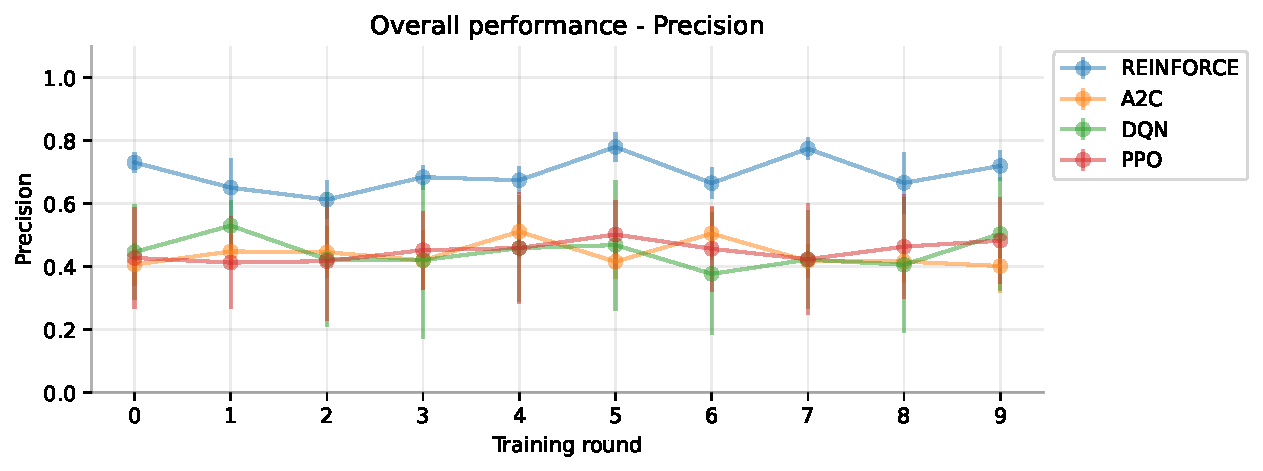
\includegraphics[width=\linewidth]{Overall_Pr.pdf}  
		\caption{Precision}
		\label{fig:tr-ovr-pr}
	\end{subfigure} \par\smallskip
	
	\begin{subfigure}{\textwidth}
		\centering
		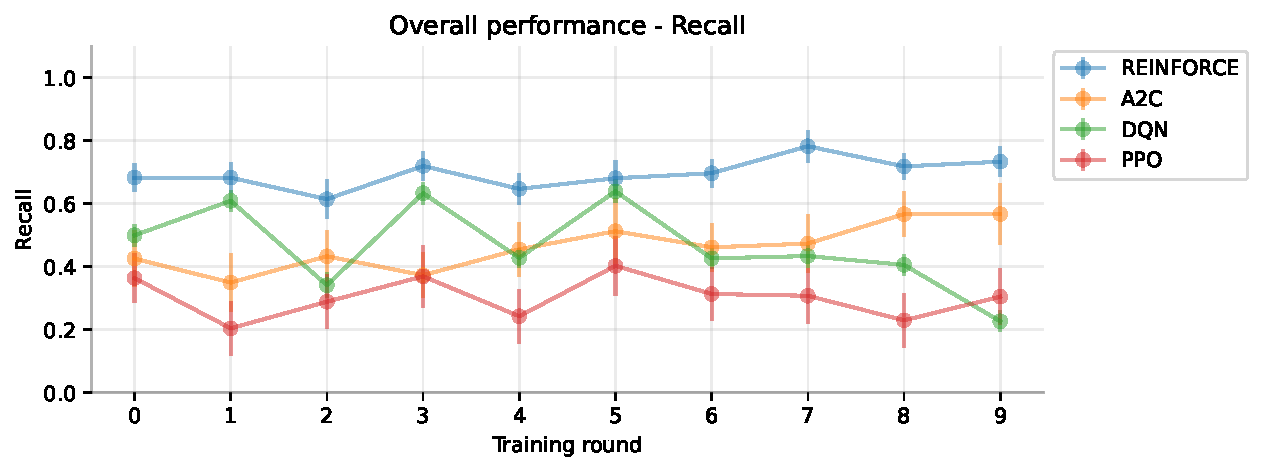
\includegraphics[width=\linewidth]{Overall_Rc.pdf}  
		\caption{Recall}
		\label{fig:tr-ovr-rc}
	\end{subfigure} \par\smallskip
	
	\begin{subfigure}{\textwidth}
		\centering
		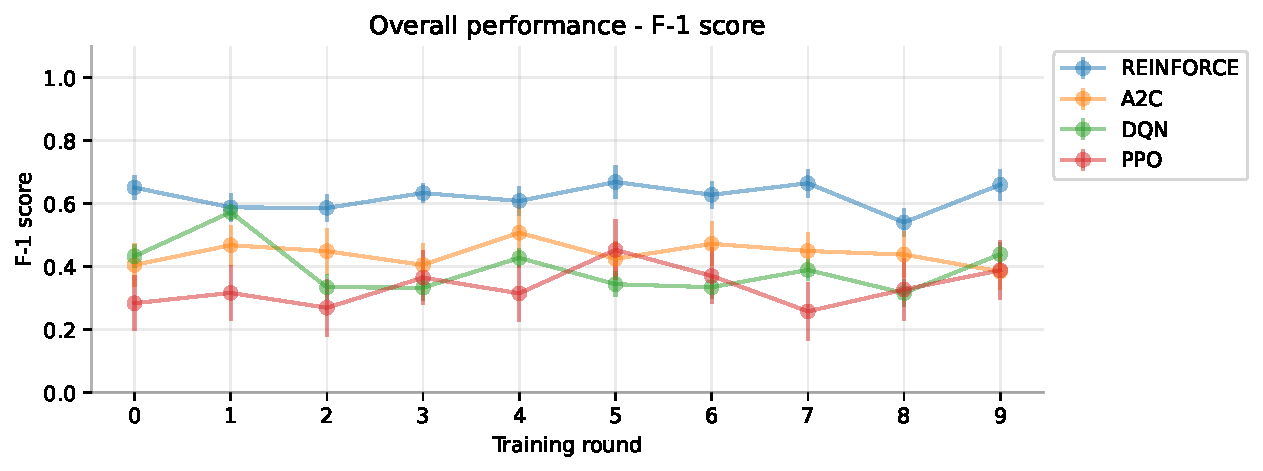
\includegraphics[width=\linewidth]{Overall_F1.pdf}  
		\caption{F1-score}
		\label{fig:tr-ovr-f1}
	\end{subfigure}
	\caption{Overall performance -- Average over 10 models}
	\label{fig:tr-overall}
\end{figure}

\begin{figure}[h]
	\begin{subfigure}{\textwidth}
		\centering
		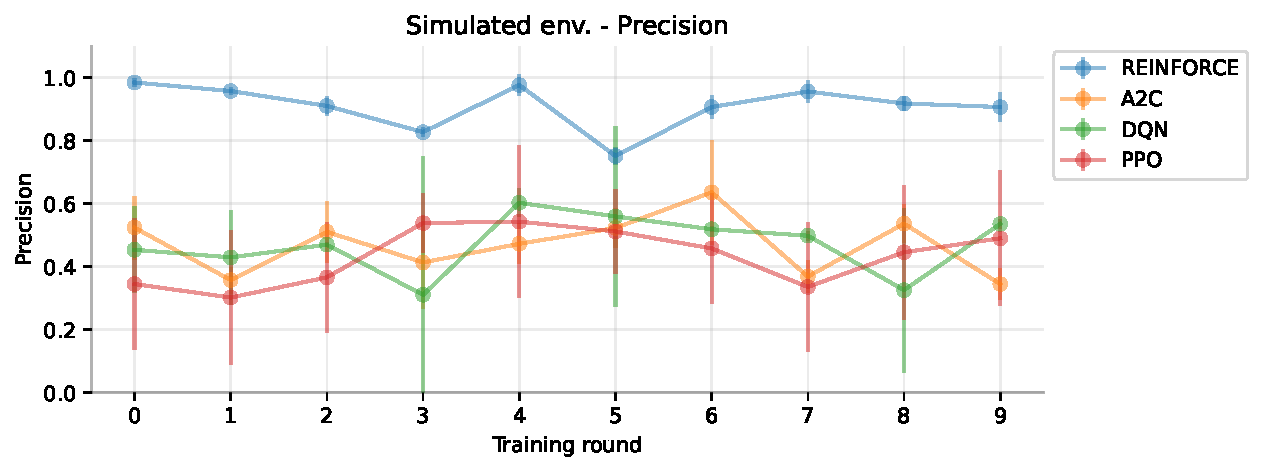
\includegraphics[width=\linewidth]{Simulated_Pr.pdf}  
		\caption{Precision}
		\label{fig:tr-sim-pr}
	\end{subfigure} \par\smallskip
	
	\begin{subfigure}{\textwidth}
		\centering
		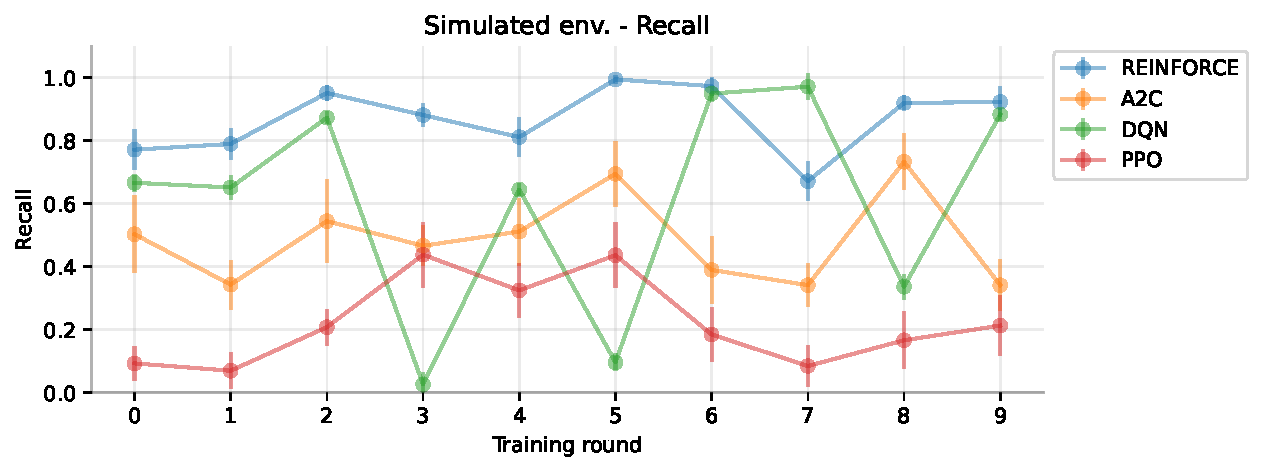
\includegraphics[width=\linewidth]{Simulated_Rc.pdf}  
		\caption{Recall}
		\label{fig:tr-sim-rc}
	\end{subfigure} \par\smallskip
	
	\begin{subfigure}{\textwidth}
		\centering
		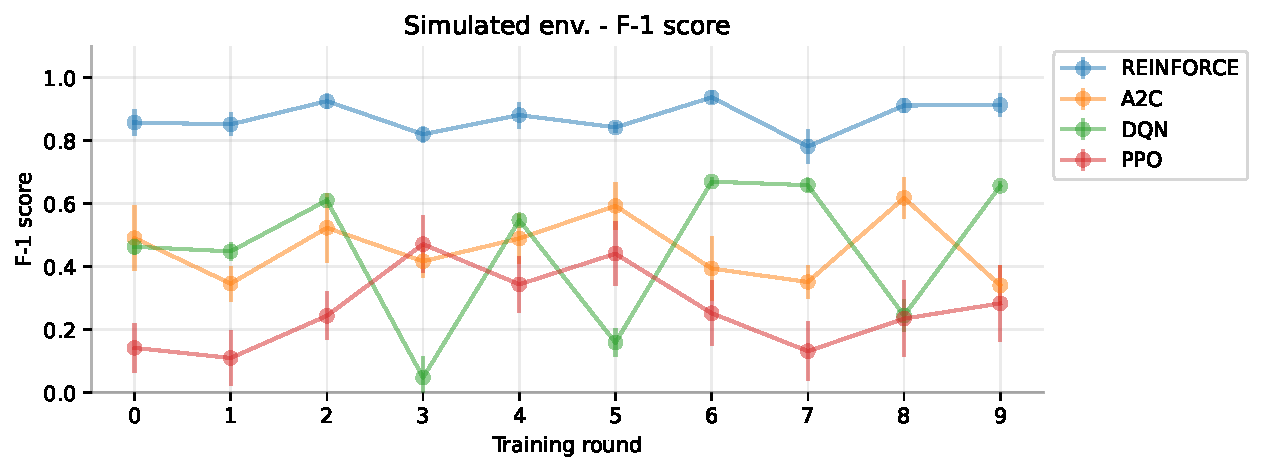
\includegraphics[width=\linewidth]{Simulated_F1.pdf}  
		\caption{F1-score}
		\label{fig:tr-sim-f1}
	\end{subfigure} \par\smallskip
	
	
	\caption{Simulated environment -- Average over 10 models}
	\label{fig:tr-sim-env}
\end{figure}

\begin{figure}[h]
	\begin{subfigure}{\textwidth}
		\centering
		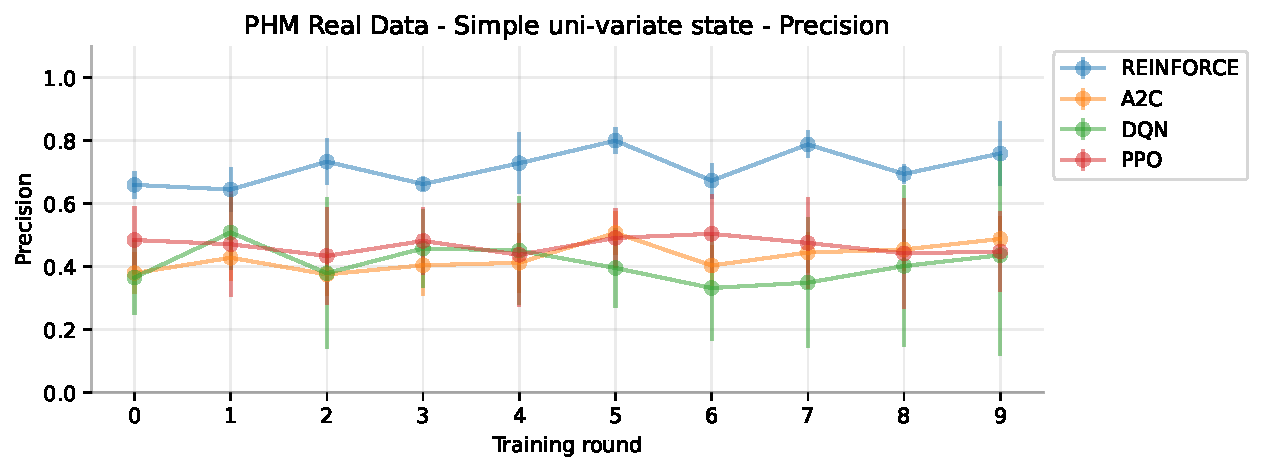
\includegraphics[width=\linewidth]{Singevariable_Pr.pdf}  
		\caption{Precision}
		\label{fig:tr-ss-pr}
	\end{subfigure} \par\smallskip
	
	\begin{subfigure}{\textwidth}
		\centering
		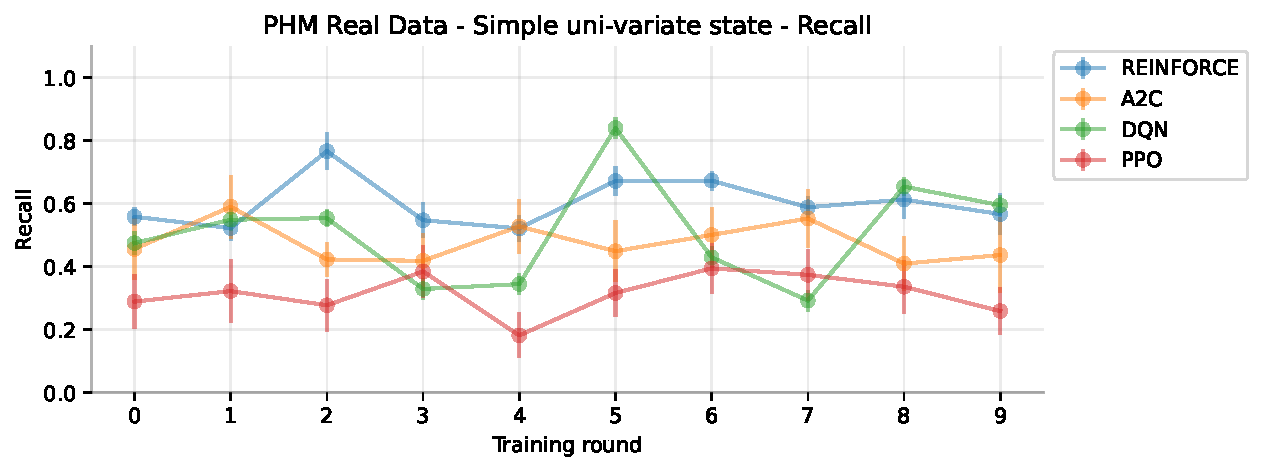
\includegraphics[width=\linewidth]{Singevariable_Rc.pdf}  
		\caption{Recall}
		\label{fig:tr-ss-rc}
	\end{subfigure} \par\smallskip
	
	\begin{subfigure}{\textwidth}
		\centering
		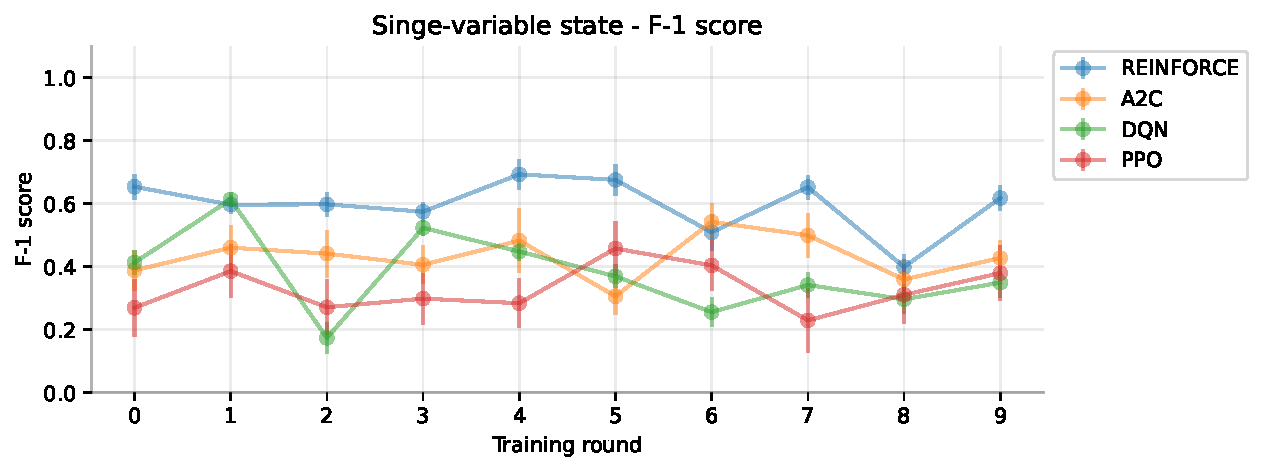
\includegraphics[width=\linewidth]{Singevariable_F1.pdf}  
		\caption{F1-score}
		\label{fig:tr-ss-f1}
	\end{subfigure} \par\smallskip
	\caption{Univariate state environment -- Average over 10 models}
	\label{fig:tr-ss-env}
\end{figure}

\begin{figure}[h]
	\begin{subfigure}{\textwidth}
		\centering
		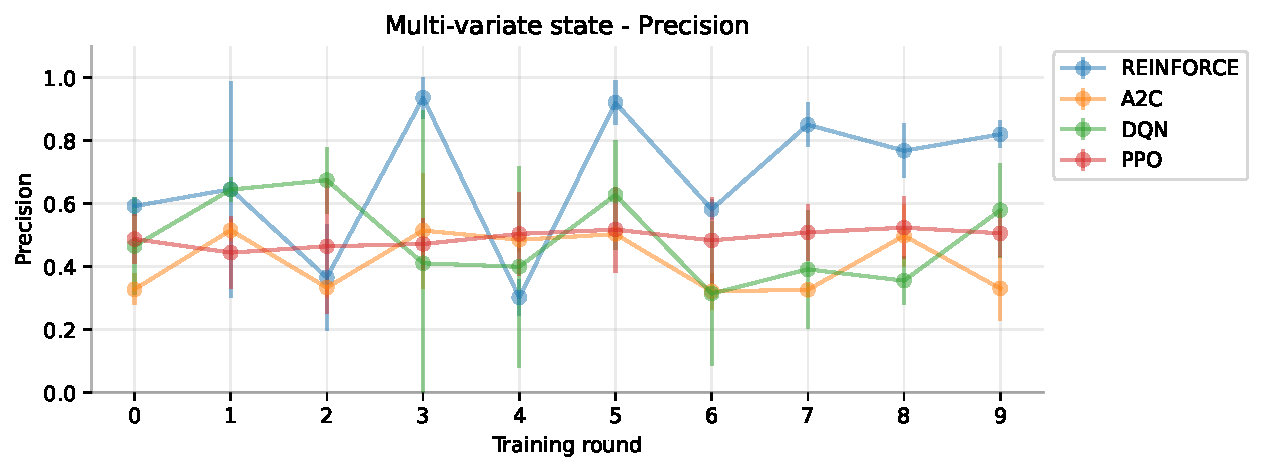
\includegraphics[width=\linewidth]{Multivariate_Pr.pdf}  
		\caption{Precision}
		\label{fig:tr-ms-pr}
	\end{subfigure} \par\smallskip
	
	\begin{subfigure}{\textwidth}
		\centering
		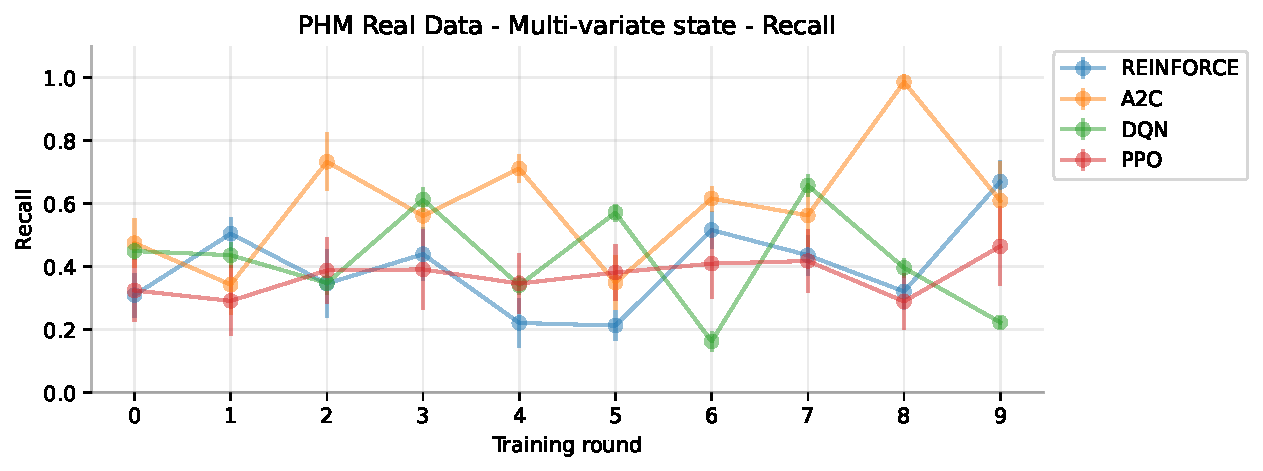
\includegraphics[width=\linewidth]{Multivariate_Rc.pdf}  
		\caption{Recall}
		\label{fig:tr-ms-rc}
	\end{subfigure} \par\smallskip
	
	\begin{subfigure}{\textwidth}
		\centering
		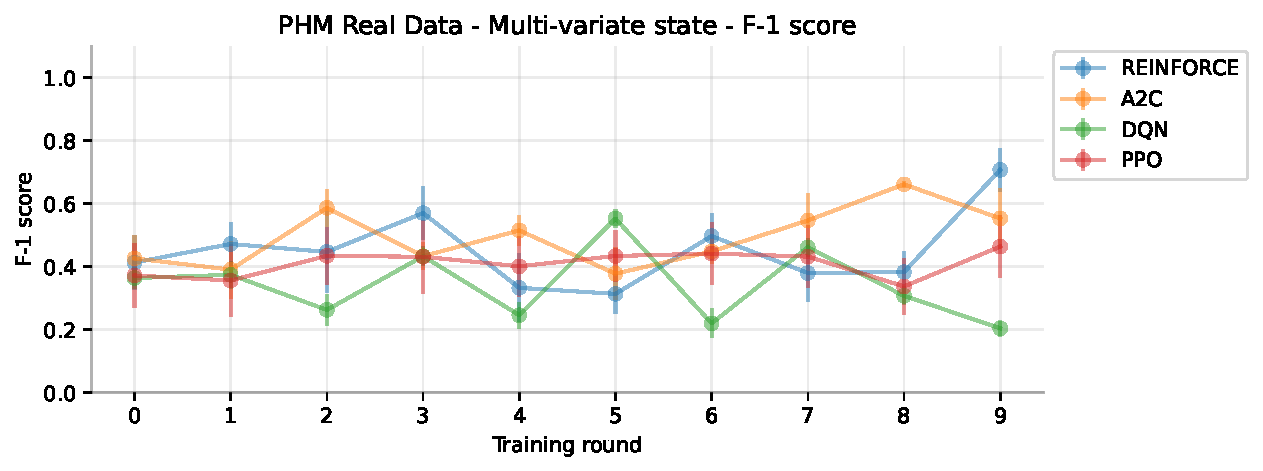
\includegraphics[width=\linewidth]{Multivariate_F1.pdf}  
		\caption{F1-score}
		\label{fig:tr-ms-f1}
	\end{subfigure} \par\smallskip
	\caption{Multivariate state environment -- Average over 10 models}
	\label{fig:tr-ms-env}
\end{figure}

%%\subsection{Detailed performance across all variants - Averaged over 10 rounds of training}
%\newgeometry{margin=1cm} % Change margins for landscape table
%\begin{landscape}\centering
%	\begin{table*}
%		\sffamily
%		\rowspace{1.3}
%		\begin{tabular}{@{}l rrrr @{\kern8pt}c rrrr @{\kern8pt}c rrrr @{\kern8pt}c rrrr@{}} \arrayrulecolor{black!40}\toprule
%			& \multicolumn{4}{c}{\textbf{REINFORCE}} & & \multicolumn{4}{c}{A2C} &
%			& \multicolumn{4}{c}{DQN} & & \multicolumn{4}{c}{PPO} \\
%			\cmidrule{2-5} \cmidrule{7-10} \cmidrule{12-15} \cmidrule{17-20}
%			Environment &Prec. &Recall &F1 &F$_\beta$0.5 & &Prec. &Recall &F1 &F$_\beta$0.5 & &Prec. &Recall &F1 &F$_\beta$0.5 & &Prec. &Recall &F1 &F$_\beta$0.5\\ \midrule
%			Simulated  - No noise &\underline{0.842} &\underline{0.878} &\underline{0.838} & \underline{0.834} & & 0.424 &0.451 &0.423 &0.421 & &0.426 &0.674 &0.471 &0.410 & &0.504 &0.200 &0.271&0.360\\
%			Simulated  - Low noise &\underline{0.777} &\underline{0.929} &\underline{0.834} & \underline{0.796} & & 0.465 &0.423 &0.409 &0.427 & &0.421 &0.338 &0.270 &0.283 & &0.482 &0.236 &0.296&0.369\\
%			Simulated  - High noise &\underline{0.798} &\underline{0.940} &\underline{0.851} & \underline{0.816} & & 0.358 &0.281 &0.256 &0.272 & &0.447 &0.519 &0.380 &0.360 & &0.514 &0.207 &0.286&0.382\\ \midrule
%			
%			PHM C01 SS - No noise &0.478 &0.363 &0.400 & 0.439 & & \underline{0.501} &0.500 &0.493 &\underline{0.496} & &0.472 &\underline{0.807} &\underline{0.568} &0.490 & &0.440 &0.417 &0.387&0.395\\
%			PHM C01 SS - Low noise &0.507 &0.311 &0.332 & 0.383 & & \underline{0.503} &\underline{0.598} &\underline{0.535} &\underline{0.513} & &0.393 &0.502 &0.351 &0.317 & &0.522 &0.338 &0.388&0.448\\
%			PHM C01 SS - High noise &\underline{0.693} &\underline{0.562} &\underline{0.579} & \underline{0.623} & & 0.266 &0.282 &0.267 &0.262 & &0.458 &0.525 &0.400 &0.384 & &0.456 &0.369 &0.372&0.400\\ \hdashline
%			
%			PHM C04 SS - No noise &\underline{0.751} &\underline{0.878} &\underline{0.784} & \underline{0.757} & & 0.487 &0.442 &0.449 &0.463 & &0.439 &0.684 &0.472 &0.411 & &0.500 &0.510 &0.469&0.473\\
%			PHM C04 SS - Low noise &\underline{0.662} &\underline{0.756} &\underline{0.672} & \underline{0.657} & & 0.409 &0.455 &0.428 &0.416 & &0.411 &0.500 &0.370 &0.341 & &0.488 &0.280 &0.324&0.386\\
%			PHM C04 SS - High noise &\underline{0.611} &\underline{0.713} &\underline{0.620} & \underline{0.598} & & 0.518 &0.607 &0.552 &0.530 & &0.358 &0.451 &0.325 &0.294 & &0.428 &0.262 &0.286&0.333\\ \hdashline
%			
%			PHM C06 SS - No noise &\underline{0.830} &\underline{0.726} &\underline{0.754} & \underline{0.792} & & 0.517 &0.509 &0.507 &0.511 & &0.360 &0.309 &0.256 &0.258 & &0.409 &0.248 &0.275&0.321\\
%			PHM C06 SS - Low noise &0.205 &0.279 &0.228 & 0.212 & & \underline{0.510} &\underline{0.577} &\underline{0.530} &\underline{0.516} & &0.434 &0.266 &0.266 &0.296 & &0.417 &0.181 &0.232&0.294\\
%			PHM C06 SS - High noise &\underline{0.709} &\underline{0.843} &\underline{0.759 }& \underline{0.726} & & 0.316 &0.324 &0.311 &0.308 & &0.449 &0.518 &0.400 &0.375 & &0.388 &0.222 &0.265&0.317\\ \midrule
%			
%			PHM C01 MS - No noise &\underline{0.835} &\underline{0.652} &\underline{0.656} & \underline{0.716} & & 0.461 &0.444 &0.397 &0.404 & &0.384 &0.558 &0.393 &0.348 & &0.513 &0.383 &0.416&0.460\\
%			PHM C04 MS - No noise &\underline{0.739} &0.255 &0.359 & \underline{0.494} & & 0.498 &\underline{0.589 }&\underline{0.490} &0.470 & &0.323 &0.209 &0.160 &0.168 & &0.499 &0.393 &0.421&0.457\\
%			PHM C06 MS - No noise &\underline{0.864} &0.356 &0.469 & \underline{0.616} & & 0.501 &\underline{0.713} &\underline{0.578} &0.527 & &0.489 &0.705 &0.529 &0.479 & &0.523 &0.488 &0.485&0.498\\
%			
%			\bottomrule
%		\end{tabular}
%		\caption{Model performance comparison all variants of the environments, over 10 rounds of training. Maximum values are underlined.}
%		\label{tbl:DetailedMetrics}
%	\end{table*}
%\end{landscape}
%\restoregeometry % Restore margins after landscape table
%\newgeometry{left=1in, top=1in, right=1in, bottom=1in}
%
%%\subsection{Super models - Detailed performance across all variants}
%\newgeometry{margin=1cm} % Change margins for landscape table
%\begin{landscape}\centering
%	\begin{table*}
%			\sffamily
%			\rowspace{1.3}
%			\begin{tabular}{@{}l rrrr c rrrr c rrrr c rrrr@{}} \arrayrulecolor{black!40}\toprule
%					& \multicolumn{4}{c}{\textbf{REINFORCE}} & & \multicolumn{4}{c}{A2C} &
%					& \multicolumn{4}{c}{DQN} & & \multicolumn{4}{c}{PPO} \\
%					\cmidrule{2-5} \cmidrule{7-10} \cmidrule{12-15} \cmidrule{17-20}
%					Environment &Prec. &Recall &F1 &F$_\beta$0.5 & &Prec. &Recall &F1 &F$_\beta$0.5 & &Prec. &Recall &F1 &F$_\beta$0.5 & &Prec. &Recall &F1 &F$_\beta$0.5\\ \midrule
%					Simulated  - No noise &\underline{0.897} &0.960 &\underline{0.926} & \underline{0.908} & & 0.500 &\underline{1.000} &0.667 &0.556 & &0.505 &0.980 &0.667 &0.560 & &0.669 &0.430 &0.518&0.597\\
%					Simulated  - Low noise &\underline{0.960} &0.945 &\underline{0.952} & \underline{0.957} & & 0.516 &\underline{1.000} &0.680 &0.571 & &0.500 &0.980 &0.662 &0.554 & &0.633 &0.460 &0.530&0.586\\
%					Simulated  - High noise &\underline{0.922} &0.990 &\underline{0.955} & \underline{0.935} & & 0.503 &\underline{1.000} &0.669 &0.558 & &0.504 &0.990 &0.668 &0.559 & &0.569 &0.355 &0.434&0.505\\\midrule
%					
%					PHM C01 SS - No noise &\underline{0.889} &0.995 &\underline{0.939} & \underline{0.908} & & 0.586 &0.625 &0.603 &0.592 & &0.647 &0.970 &0.776 &0.693 & &0.543 &\underline{1.000} &0.703&0.597\\
%					PHM C01 SS - Low noise &\underline{0.988} &0.765 &\underline{0.861} & \underline{0.932} & & 0.499 &0.995 &0.664 &0.554 & &0.504 &\underline{0.990} &0.668 &0.559 & &0.623 &0.740 &0.675&0.643\\
%					PHM C01 SS - High noise &\underline{0.850} &0.970 &\underline{0.905} & \underline{0.871} & & 0.521 &0.680 &0.588 &0.546 & &0.505 &\underline{0.985} &0.668 &0.560 & &0.520 &0.725 &0.604&0.551\\\hdashline
%					
%					PHM C04 SS - No noise &\underline{0.811} &\underline{1.000} &\underline{0.895} & \underline{0.842} & & 0.536 &0.645 &0.583 &0.554 & &0.501 &0.965 &0.660 &0.554 & &0.579 &0.895 &0.702&0.622\\
%					PHM C04 SS - Low noise &\underline{0.798} &0.980 &\underline{0.879} & \underline{0.829} & & 0.556 &0.665 &0.603 &0.573 & &0.734 &\underline{0.990} &0.843 &0.774 & &0.546 &0.660 &0.596&0.565\\
%					PHM C04 SS - High noise &\underline{0.708} &0.840 &\underline{0.767} & \underline{0.730} & & 0.521 &0.835 &0.641 &0.563 & &0.511 &\underline{0.985} &0.672 &0.565 & &0.517 &0.820 &0.633&0.558\\\hdashline
%					
%					PHM C06 SS - No noise &\underline{1.000} &\underline{0.895} &\underline{0.944} & \underline{0.977} & & 0.520 &0.680 &0.587 &0.545 & &0.935 &0.975 &0.954 &0.942 & &0.587 &0.650 &0.615&0.597\\
%					PHM C06 SS - Low noise &\underline{0.943} &0.795 &\underline{0.861} & \underline{0.908} & & 0.501 &\underline{1.000} &0.668 &0.557 & &0.961 &0.725 &0.826 &0.901 & &0.552 &0.370 &0.438&0.497\\
%					PHM C06 SS - High noise &0.821 &0.845 &0.831 & 0.825 & & 0.540 &0.755 &0.628 &0.572 & &\underline{0.980} &\underline{0.960}&\underline{0.969} &\underline{0.976} & &0.521 &0.615 &0.564&0.537\\\midrule
%					
%					PHM C01 MS - No noise &\underline{0.827} &0.995 &\underline{0.903} & \underline{0.856} & & 0.500 &\underline{1.000} &0.667 &0.556 & &0.505 &0.985 &0.668 &0.560 & &0.512 &0.595 &0.549&0.526\\
%					PHM C04 MS - No noise &\underline{0.910}&0.425 &0.577 & \underline{0.738} & & 0.500 &\underline{1.000} &\underline{0.667} &0.556 & &0.501 &0.975 &0.662 &0.555 & &0.501 &0.635 &0.558&0.522\\
%					PHM C06 MS - No noise &\underline{0.934} &0.865 &\underline{0.896} & \underline{0.918} & & 0.500 &\underline{1.000} &0.667 &0.556 & &0.969 &0.600 &0.741 &0.863 & &0.497 &0.690 &0.577&0.526\\			
%					\bottomrule
%				\end{tabular}
%			\caption{Super Models: Best models selected over 10 rounds of training. Maximum performance values are underlined.}
%			\label{tbl:SuperModels}
%		\end{table*}
%\end{landscape}
%% Restore margins after landscape table
%\restoregeometry 
%\newgeometry{left=1in, top=1in, right=1in, bottom=1in}
\end{appendices}

%% References
\singlespacing
\bibliographystyle{plainnat}
\bibliography{ES_bibliography}
\end{document}
